% Options for packages loaded elsewhere
\PassOptionsToPackage{unicode}{hyperref}
\PassOptionsToPackage{hyphens}{url}
\PassOptionsToPackage{dvipsnames,svgnames,x11names}{xcolor}
\documentclass[
  10pt,
  letterpaper,
]{article}
\usepackage{xcolor}
\usepackage[margin=1in]{geometry}
\usepackage{amsmath,amssymb}
\setcounter{secnumdepth}{-\maxdimen} % remove section numbering
\usepackage{iftex}
\ifPDFTeX
  \usepackage[T1]{fontenc}
  \usepackage[utf8]{inputenc}
  \usepackage{textcomp} % provide euro and other symbols
\else % if luatex or xetex
  \usepackage{unicode-math} % this also loads fontspec
  \defaultfontfeatures{Scale=MatchLowercase}
  \defaultfontfeatures[\rmfamily]{Ligatures=TeX,Scale=1}
\fi
\usepackage{lmodern}
\ifPDFTeX\else
  % xetex/luatex font selection
\fi
% Use upquote if available, for straight quotes in verbatim environments
\IfFileExists{upquote.sty}{\usepackage{upquote}}{}
\IfFileExists{microtype.sty}{% use microtype if available
  \usepackage[]{microtype}
  \UseMicrotypeSet[protrusion]{basicmath} % disable protrusion for tt fonts
}{}
\usepackage{setspace}
\makeatletter
\@ifundefined{KOMAClassName}{% if non-KOMA class
  \IfFileExists{parskip.sty}{%
    \usepackage{parskip}
  }{% else
    \setlength{\parindent}{0pt}
    \setlength{\parskip}{6pt plus 2pt minus 1pt}}
}{% if KOMA class
  \KOMAoptions{parskip=half}}
\makeatother
\usepackage{longtable,booktabs,array}
\newcounter{none} % for unnumbered tables
\usepackage{calc} % for calculating minipage widths
% Correct order of tables after \paragraph or \subparagraph
\usepackage{etoolbox}
\makeatletter
\patchcmd\longtable{\par}{\if@noskipsec\mbox{}\fi\par}{}{}
\makeatother
% Allow footnotes in longtable head/foot
\IfFileExists{footnotehyper.sty}{\usepackage{footnotehyper}}{\usepackage{footnote}}
\makesavenoteenv{longtable}
\usepackage{graphicx}
\makeatletter
\newsavebox\pandoc@box
\newcommand*\pandocbounded[1]{% scales image to fit in text height/width
  \sbox\pandoc@box{#1}%
  \Gscale@div\@tempa{\textheight}{\dimexpr\ht\pandoc@box+\dp\pandoc@box\relax}%
  \Gscale@div\@tempb{\linewidth}{\wd\pandoc@box}%
  \ifdim\@tempb\p@<\@tempa\p@\let\@tempa\@tempb\fi% select the smaller of both
  \ifdim\@tempa\p@<\p@\scalebox{\@tempa}{\usebox\pandoc@box}%
  \else\usebox{\pandoc@box}%
  \fi%
}
% Set default figure placement to htbp
\def\fps@figure{htbp}
\makeatother
\setlength{\emergencystretch}{3em} % prevent overfull lines
\providecommand{\tightlist}{%
  \setlength{\itemsep}{0pt}\setlength{\parskip}{0pt}}
\usepackage{bookmark}
\IfFileExists{xurl.sty}{\usepackage{xurl}}{} % add URL line breaks if available
\urlstyle{same}
\hypersetup{
  colorlinks=true,
  linkcolor={black},
  filecolor={Maroon},
  citecolor={Blue},
  urlcolor={blue},
  pdfcreator={LaTeX via pandoc}}

\author{}
\date{}

\usepackage{caption}
\begin{document}

\setstretch{1.15}
\section{Leakage-Safe Multi-Seed Evaluation of Published BU-Net
Components for Resource-Constrained 2D Glioma
Segmentation}\label{leakage-safe-multi-seed-evaluation-of-published-bu-net-components-for-resource-constrained-2d-glioma-segmentation}

Taha Berk Terekli\textsuperscript{1}, Livanur Mengeş\textsuperscript{2},
Volkan Yusuf Hal\textsuperscript{3}, Ali Emre Döşer\textsuperscript{4}

\textsuperscript{1} Department of Mathematics, Yıldız Technical
University, Istanbul, Turkey\\
\textsuperscript{2} Department of Computer Engineering, Istanbul Beykent
University, Istanbul, Turkey\\
\textsuperscript{3} Department of Software Engineering, Istanbul Beykent
University, Istanbul, Turkey\\
\textsuperscript{4} Department of Computer Engineering, Haliç
University, Istanbul, Turkey

\textbf{Corresponding author:} Taha Berk Terekli\\
\textbf{Running title:} Controlled evaluation of BU-Net components\\
\textbf{Article type:} Original research - methodological evaluation

\subsection{Abstract}\label{abstract}

\textbf{Background:} Architectural comparisons in glioma segmentation
are vulnerable to patient leakage, inconsistent training budgets,
incomplete attribution, and selective reporting. We evaluated previously
published BU-Net components under a single guarded protocol rather than
proposing a new architecture.

\textbf{Methods:} BraTS 2020 training cases formed the canonical labeled
cohort. BraTS 2019 was used only to audit identity overlap. All 369
canonical patients were split at patient level into 258 training, 37
validation, and 74 internal held-out test cases. A standard 2D U-Net,
the published BU-Net reimplementation with residual extended skip (RES)
and wide context (WC) modules, and U-Net+RES were trained with identical
preprocessing, loss, optimization, and 2,000-step per-run limits.
Development screening preceded a five-seed finalist stage. The test
manifest was opened once after candidate and analysis freezing. The
primary outcome was patient-level mean Dice across whole tumor, tumor
core, and enhancing tumor. Three paired contrasts used 10,000 bootstrap
resamples, 100,000 sign-flip permutations, and Holm correction.

\textbf{Results:} On the internal held-out test subset, mean regional
Dice was 0.736 for standard U-Net, 0.752 for BU-Net, and 0.756 for
U-Net+RES. Relative to standard U-Net, paired differences were +0.017
for BU-Net (95\% CI +0.005 to +0.030; Holm p=0.014) and +0.020 for
U-Net+RES (95\% CI +0.008 to +0.034; Holm p=0.004). BU-Net was lower
than U-Net+RES by 0.004 (95\% CI -0.008 to -0.000; Holm p=0.050). BU-Net
used 8.385 million parameters versus 4.450 million for U-Net+RES and had
higher median latency and peak allocated memory.

\textbf{Conclusions:} Under this bounded 2D protocol, the published RES
component was associated with a small improvement over standard U-Net.
Adding WC in the full BU-Net did not improve the primary endpoint over
RES alone and increased resource demand. These internal, single-dataset
findings do not establish clinical utility, external generalization, or
superiority over 3D, transformer, or self-configuring systems.

\textbf{Keywords:} brain tumor segmentation; BraTS; U-Net; BU-Net;
reproducibility; patient-level evaluation; resource profiling

\pagebreak

\subsection{1. Introduction}\label{introduction}

Glioma segmentation supports quantitative analysis of multimodal
magnetic resonance imaging (MRI), but model rankings can be distorted by
experimental design. Slice-level partitioning can place images from one
patient in multiple subsets. Reusing overlapping BraTS editions can
duplicate subjects. A comparison can also favor one architecture through
a different loss, augmentation policy, run duration, or stopping rule.
Finally, an overlap score alone does not describe boundary error, lesion
detection, failure modes, or computational demand.

The BraTS benchmark standardized multimodal glioma MRI and the
evaluation of whole tumor (WT), tumor core (TC), and enhancing tumor
(ET) {[}1-4{]}. U-Net remains a useful reference architecture {[}5{]}.
Rehman et al.~later described BU-Net, a 2D U-Net modification containing
residual extended skip (RES) and wide context (WC) modules {[}6{]}.
These modules are prior work; we do not claim either component as novel.
Our question is narrower: what evidence do RES and WC provide when
implemented in one codebase and evaluated with matched data, training,
statistical, and resource protocols?

Contemporary segmentation systems include self-configuring pipelines and
volumetric transformer designs {[}9,14,15{]}. They are important
context, but they were not trained here. Comparing our internal scores
with literature values produced under different cohorts and protocols
would not be a controlled benchmark. We therefore position this work as
a component and reproducibility study within a 2D U-Net family.

The study makes four contributions:

\begin{enumerate}
\def\labelenumi{\arabic{enumi}.}
\tightlist
\item
  a content-based audit of the overlap between BraTS 2019 and BraTS 2020
  before selecting one canonical cohort;
\item
  a patient-level development and test workflow with a frozen, one-time
  internal-test access event;
\item
  a multi-seed, matched-protocol evaluation of standard U-Net,
  U-Net+RES, and the full BU-Net reimplementation; and
\item
  artifact-derived statistical, resource, subgroup, and qualitative
  reports released with executable checks.
\end{enumerate}

No contribution is framed as a new network block, clinical device, or
state-of-the-art result.

\subsection{2. Related work}\label{related-work}

BraTS combines T1, post-contrast T1, T2, and FLAIR MRI with expert tumor
annotations {[}1-4{]}. The official tasks define WT as labels 1, 2, and
4; TC as labels 1 and 4; and ET as label 4 {[}2{]}. Dice and
95th-percentile Hausdorff distance (HD95) are established challenge
measures, but each captures a different property of the segmentation.

U-Net introduced an encoder-decoder design with skip connections for
biomedical segmentation {[}5{]}. BU-Net retained the 2D U-Net form while
adding RES modules to the skip pathways and a WC module at the
bottleneck {[}6{]}. The large separable kernels in these modules aim to
increase contextual support. Because RES and WC originated in BU-Net,
the present implementation and all component names are attributed to
Rehman et al.

Loss design also matters for imbalanced lesions. Tversky and focal
Tversky objectives modify the relative weighting of false-positive and
false-negative errors {[}7,8{]}. We screened these objectives under the
same development protocol rather than assigning different losses to
different final models.

Methodological guidance recommends choosing metrics for the task,
preserving the correct unit of analysis, reporting the split level,
declaring primary outcomes, and making software available {[}10,12{]}.
We therefore used the patient as the statistical unit, treated secondary
endpoints as estimation-only analyses, and retained undefined or
infinite outcomes instead of silently replacing them. Surface Dice was
included at a predeclared 1 mm tolerance {[}11{]}. That tolerance is an
analytic setting, not a claim of clinical acceptability or interobserver
calibration.

\subsection{3. Materials and methods}\label{materials-and-methods}

\subsubsection{3.1 Study design and reporting
scope}\label{study-design-and-reporting-scope}

This was a retrospective computational study of a public, de-identified
challenge dataset. The workflow was organized into sequential gates:
data integrity and identity audit; patient-level split; preprocessing
and evaluator validation; model and loss implementation tests;
single-seed development screening; multi-seed confirmation; analysis
freezing; one guarded internal-test evaluation; and artifact-derived
reporting. CLAIM 2024 informed the reporting checklist {[}12{]}.

The study did not use the official BraTS 2020 validation set because its
reference labels were withheld. In this paper, ``internal held-out test
subset'' refers only to the labeled partition created from the BraTS
2020 training cohort.

\begin{figure}
\centering
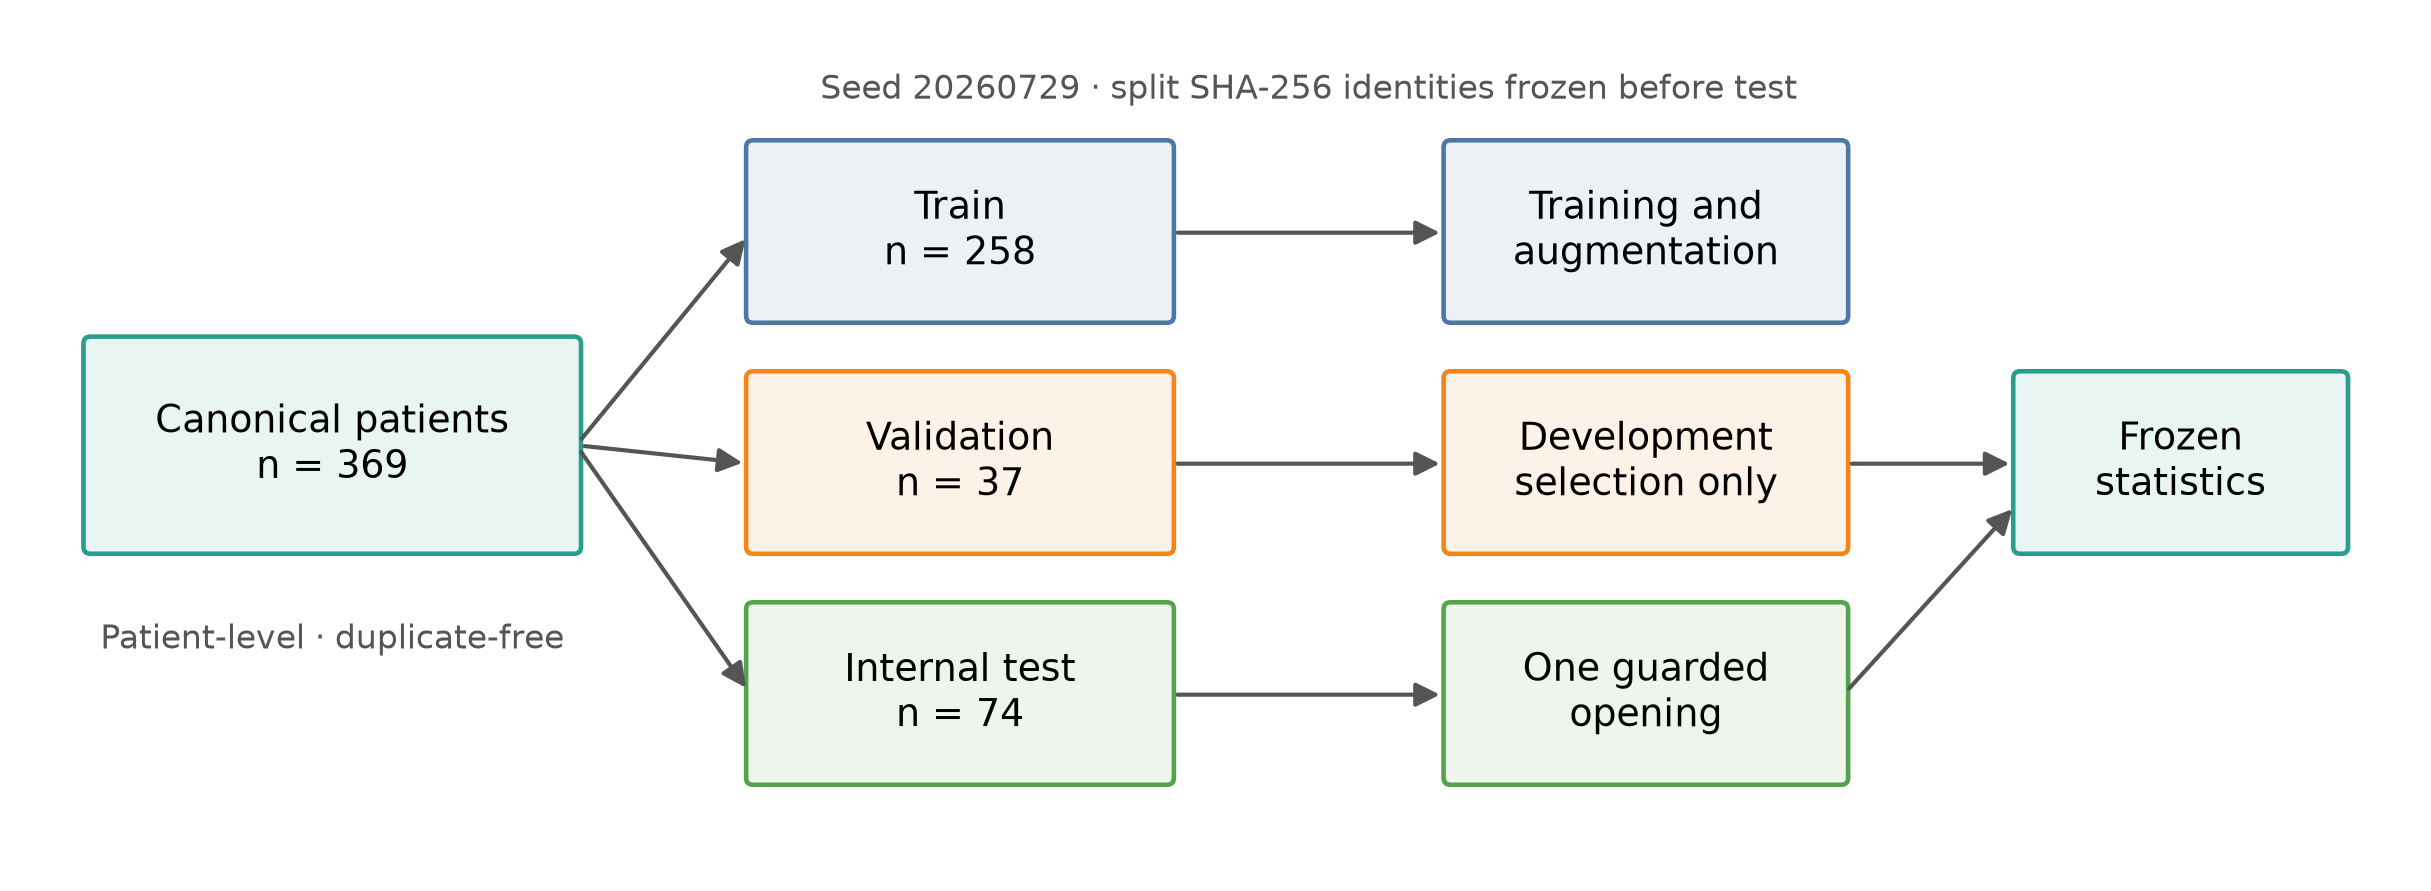
\includegraphics[width=0.92\linewidth,height=\textheight,keepaspectratio,alt={Figure 1. Gated development, freezing, and one-time internal-test analysis flow.}]{../figures/final/fig02_split_and_analysis_flow.png}
\caption{Gated development, freezing, and one-time
internal-test analysis flow.}\label{fig:flow}
\end{figure}

\subsubsection{3.2 Cohort audit, canonicalization, and
splitting}\label{cohort-audit-canonicalization-and-splitting}

We inventoried all expected modalities and segmentations by patient and
computed file- and image-content signatures. BraTS 2020 training was
selected as the canonical labeled cohort. BraTS 2019 contributed no
additional training observation and was used only for identity and
duplicate auditing.

The audit found 335 complete BraTS 2019 cases and 369 complete BraTS
2020 cases. All 335 BraTS 2019 patients mapped to BraTS 2020 by image
content; 34 cases were new in the 2020 edition. The mapped image
modalities were content-equivalent. One mapped segmentation differed by
2 voxels, which was recorded as an annotation revision rather than a new
patient. The canonical cohort therefore contained 369 unique patients.

Patients, not slices, were partitioned with seed 20260729. The selected
candidate minimized imbalance across grade, ET presence, and WT-volume
strata while satisfying frozen tolerances. Patient identifiers did not
overlap between subsets.

\textbf{Table 1. Cohort characteristics by patient-level partition.}

{\def\LTcaptype{none} % do not increment counter
\begin{longtable}[]{@{}
  >{\raggedright\arraybackslash}p{(\linewidth - 10\tabcolsep) * \real{0.1667}}
  >{\raggedright\arraybackslash}p{(\linewidth - 10\tabcolsep) * \real{0.1667}}
  >{\raggedright\arraybackslash}p{(\linewidth - 10\tabcolsep) * \real{0.1667}}
  >{\raggedright\arraybackslash}p{(\linewidth - 10\tabcolsep) * \real{0.1667}}
  >{\raggedright\arraybackslash}p{(\linewidth - 10\tabcolsep) * \real{0.1667}}
  >{\raggedright\arraybackslash}p{(\linewidth - 10\tabcolsep) * \real{0.1667}}@{}}
\toprule\noalign{}
\begin{minipage}[b]{\linewidth}\raggedright
Partition
\end{minipage} & \begin{minipage}[b]{\linewidth}\raggedright
Patients
\end{minipage} & \begin{minipage}[b]{\linewidth}\raggedright
HGG
\end{minipage} & \begin{minipage}[b]{\linewidth}\raggedright
LGG
\end{minipage} & \begin{minipage}[b]{\linewidth}\raggedright
ET present
\end{minipage} & \begin{minipage}[b]{\linewidth}\raggedright
WT volume median (IQR), mm3
\end{minipage} \\
\midrule\noalign{}
\endhead
\bottomrule\noalign{}
\endlastfoot
Train & 258 & 204 & 54 & 239 & 90936.0 (50321.0-144849.5) \\
Validation & 37 & 30 & 7 & 34 & 89516.0 (52898.0-149466.0) \\
Internal test & 74 & 59 & 15 & 69 & 89554.0 (51805.8-141632.2) \\
\end{longtable}
}

\begin{figure}
\centering
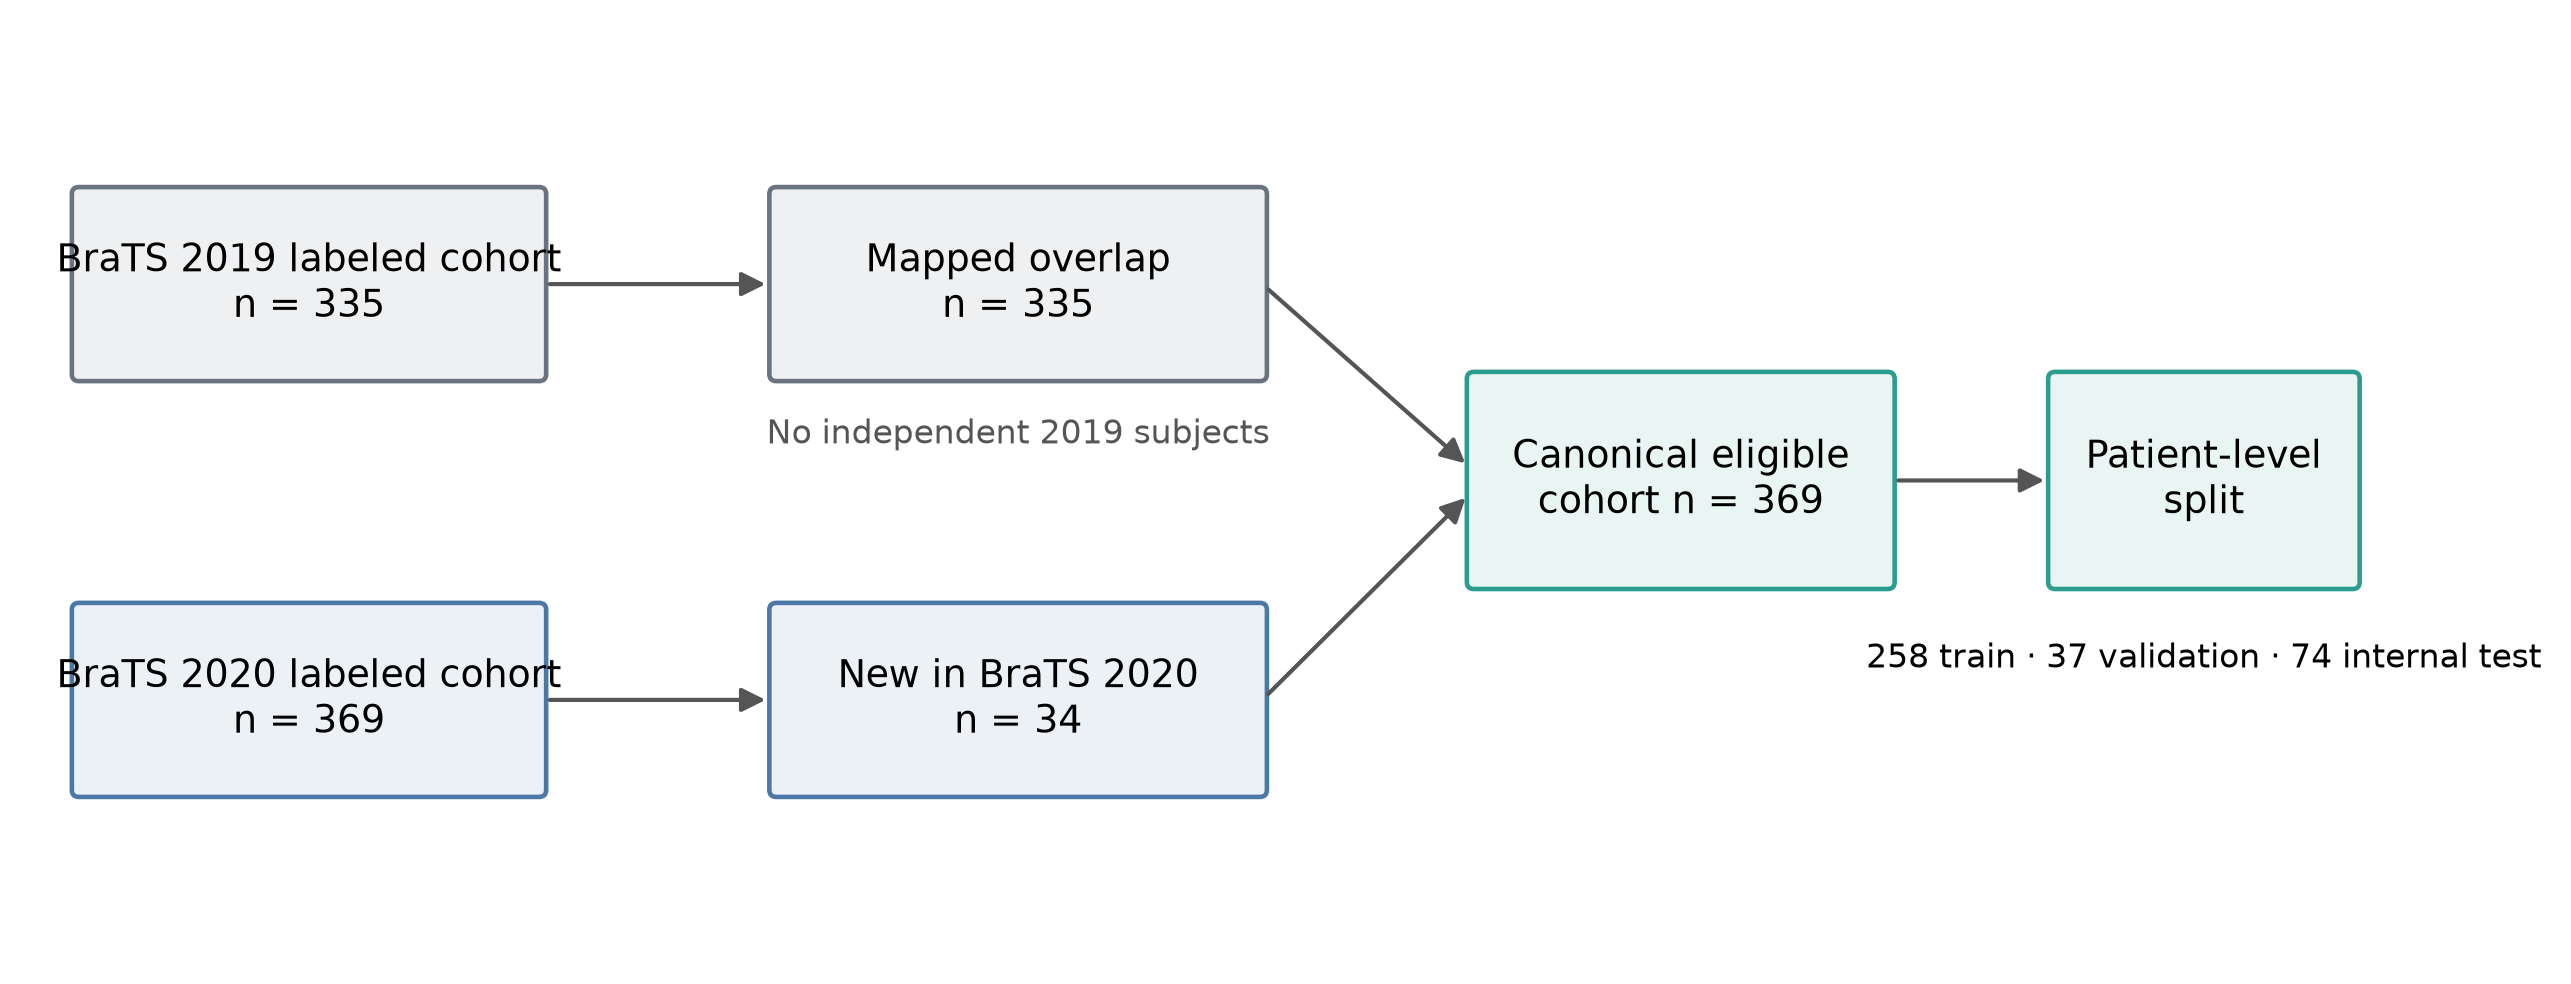
\includegraphics[width=0.92\linewidth,height=\textheight,keepaspectratio,alt={Figure 2. Cohort identity audit and canonical patient flow.}]{../figures/final/fig01_cohort_flow.png}
\caption{Cohort identity audit and canonical patient
flow.}\label{fig:cohort}
\end{figure}

\subsubsection{3.3 MRI preprocessing and
sampling}\label{mri-preprocessing-and-sampling}

Each case used T1, T1ce, T2, and FLAIR in that channel order. Volumes
supplied by BraTS were co-registered, skull stripped, and sampled
axially at 240 x 240 pixels. For each patient and modality, nonzero
voxels were standardized with that volume's mean and standard deviation.
Intensity clipping was disabled.

Training sampled 16 slices per patient per epoch; the probability of
selecting a tumor-containing slice was 0.67 and at least one tumor voxel
defined a positive slice. Spatial augmentation used independent flips
with probability 0.5 and rotations by multiples of 90 degrees.
Per-modality intensity augmentation, applied with probability 0.5, used
scale 0.9-1.1 and shift -0.1 to 0.1 in standardized units. Validation
and test evaluation traversed all slices, including empty slices,
deterministically. Cached arrays were memory-mapped outside the raw-data
roots.

\subsubsection{3.4 Architectures and
attribution}\label{architectures-and-attribution}

All candidates accepted four MRI channels and produced four logits
representing background and BraTS labels 1, 2, and 4. The common encoder
widths were 16, 32, 64, and 128, followed by a 256-channel bottleneck.
Batch normalization and dropout probability 0.3 were shared.

Standard U-Net used ordinary encoder-decoder skip connections. U-Net+RES
added the published BU-Net RES pathways but omitted WC. The full BU-Net
reimplementation combined RES with the published WC bottleneck module.
RES used separable N x 1 and 1 x N branches with N in 9, 11, 13, and 15
across resolution levels, followed by fusion convolutions. WC used two
oppositely ordered separable 15-pixel paths whose outputs were summed.
Figure 3 identifies publication provenance directly.

The implementation followed the BU-Net prose where the original
schematic was ambiguous. Deliberate implementation choices were four
mutually exclusive output classes, base width 16, the stated dropout
placement, and no imported external code. These choices make the present
work a reimplementation study, not an exact reproduction of the original
paper.

\begin{figure}
\centering
\includegraphics[width=0.92\linewidth,height=\textheight,keepaspectratio,alt={Figure 3. Compared 2D architectures. RES and WC are published BU-Net components from Rehman et al.~{[}6{]}.}]{../figures/final/fig03_model_architectures.png}
\caption{Compared 2D architectures. RES and WC are published
BU-Net components from Rehman et al.~{[}6{]}.}\label{fig:architectures}
\end{figure}

\subsubsection{3.5 Loss function and development
screen}\label{loss-function-and-development-screen}

The selected loss was an equal-weight combination of channel-wise binary
cross-entropy (BCE) and foreground focal Tversky loss (FTL):

\[
\mathcal{L} = 0.5\,\mathcal{L}_{BCE} + 0.5\,\mathcal{L}_{FTL},
\]

\[
\mathcal{L}_{FTL} =
\frac{1}{|C_f|}\sum_{c\in C_f}
\left(1-
\frac{TP_c+\epsilon}{TP_c+\alpha FP_c+\beta FN_c+\epsilon}
\right)^\gamma ,
\]

where \(C_f\) contains the three foreground classes, \(\alpha=0.3\),
\(\beta=0.7\), \(\gamma=0.75\), and \(\epsilon=10^{-5}\). BCE used
sigmoid probabilities and one-hot targets; FTL used softmax
probabilities. Inference used argmax over the four output classes. No
class weights were applied.

The development screen evaluated six architecture arms and seven loss
arms once each on the validation subset. Its role was shortlisting, not
hypothesis testing or reporting a generalization estimate.

\textbf{Table 2. Single-seed architecture development screen (n=37
validation patients).}

{\def\LTcaptype{none} % do not increment counter
\begin{longtable}[]{@{}lll@{}}
\toprule\noalign{}
Architecture arm & Mean regional Dice & Eliminated \\
\midrule\noalign{}
\endhead
\bottomrule\noalign{}
\endlastfoot
BU-Net & 0.751 & no \\
Residual-block U-Net & 0.728 & yes \\
Residual-block U-Net+WC & 0.741 & no \\
Standard U-Net & 0.721 & yes \\
U-Net+RES & 0.745 & no \\
U-Net+WC & 0.741 & no \\
\end{longtable}
}

\textbf{Table 3. Single-seed loss development screen (n=37 validation
patients).}

{\def\LTcaptype{none} % do not increment counter
\begin{longtable}[]{@{}lll@{}}
\toprule\noalign{}
Loss arm & Mean regional Dice & Eliminated \\
\midrule\noalign{}
\endhead
\bottomrule\noalign{}
\endlastfoot
Cross-entropy + soft Dice & 0.721 & yes \\
Binary cross-entropy & 0.623 & yes \\
Binary cross-entropy + focal Tversky & 0.744 & no \\
Binary cross-entropy + soft Dice & 0.711 & yes \\
Cross-entropy & 0.700 & yes \\
Focal Tversky & 0.245 & yes \\
Soft Dice & 0.238 & yes \\
\end{longtable}
}

\subsubsection{3.6 Matched training and multi-seed
confirmation}\label{matched-training-and-multi-seed-confirmation}

Every reportable run used the same Apple M1 Max MPS device, inputs,
batch size 16, AdamW optimizer, learning rate 0.001, weight decay
0.00001, augmentation, and loss. Mixed precision and pretraining were
disabled. The realized bounded protocol stopped each run at 2,000
optimizer steps or 0.5 accelerator-hours, whichever occurred first. A
200-step linear warmup preceded cosine decay to 0.01 of the initial
rate. Validation occurred at step 2,000, and the highest patient-level
mean regional Dice checkpoint was retained.

Three seeds (3 per candidate) confirmed standard U-Net, BU-Net,
U-Net+RES, and U-Net+WC. U-Net+WC was eliminated by the predeclared
rule. BU-Net and U-Net+RES then received two additional seeds each.
Five-seed validation means were 0.743 and 0.740, respectively; the
U-Net+RES minus BU-Net paired difference was -0.003 (95\% bootstrap CI
-0.012 to +0.004). Because this interval included zero, the development
ranking was not interpreted as superiority. Standard U-Net, BU-Net, and
U-Net+RES were frozen for internal-test evaluation.

\subsubsection{3.7 Guarded internal-test
evaluation}\label{guarded-internal-test-evaluation}

Before test access, candidate identities, 13 checkpoint hashes, the
split hashes, the endpoint, three paired contrasts, inference rules, and
statistical procedures were frozen. Test evaluation required an explicit
authorization flag and an append-only access log. The test manifest was
opened once. No checkpoint, threshold, post-processing stage, or
model-selection decision changed afterward.

For each candidate, per-seed endpoint values were averaged within
patient before patient-level statistical inference. No test-time
augmentation or post-processing was used.

\subsubsection{3.8 Outcomes and metric
rules}\label{outcomes-and-metric-rules}

The primary outcome was each patient's arithmetic mean of WT, TC, and ET
Dice. Region Dice values were also reported separately. Secondary
estimates included HD95, surface Dice at 1 mm, lesion recall, lesion
precision, lesion-wise Dice, false-positive lesion count, and relative
volume error.

Lesions used 26-connectivity with a one-voxel minimum. Predicted and
reference lesions were paired by maximum-total-IoU matching. If both
masks were empty, overlap and surface Dice were 1 and HD95 was 0 mm; if
only one mask was empty, overlap and surface Dice were 0 and HD95 was
infinity. Undefined rates remained missing. Tables state finite
denominators and infinity counts where applicable.

\subsubsection{3.9 Statistical analysis}\label{statistical-analysis}

The patient was the only inferential unit. For each candidate, 95\%
confidence intervals used 10,000 patient-level bootstrap resamples with
seed 20260729. Three frozen paired comparisons of mean regional Dice
were tested with 100,000 two-sided sign-flip permutations using seed
20260730. Holm's sequential procedure controlled the family-wise error
rate at 0.05 {[}13{]}. We report paired mean differences, bootstrap
intervals, paired standardized effect \(d_z\), raw p values, and
Holm-adjusted p values. Regional and secondary endpoints were
estimation-only; no unplanned multiplicity-adjusted claims were made.

Grade, reference ET presence, and training-derived WT burden tertiles
were exploratory. The ET-absent group was descriptive because it
contained only five patients.

\subsubsection{3.10 Resource profiling and
reproducibility}\label{resource-profiling-and-reproducibility}

Parameter counts and multiply-accumulate operations (MACs) were computed
from the implemented models at a 4 x 240 x 240 slice input. One MAC was
reported as two floating-point operations (FLOPs). Per-volume inference
latency and allocated memory were measured on the same Apple M1 Max host
and summarized across seeds. Development accelerator-hours were retained
from each run. These measurements compare the present implementations on
one host; they are not deployment benchmarks.

All tables and figures were generated from machine-readable run
artifacts. A tracked manifest records hashes for reportable files. A
clean-clone audit rebuilt the Gate 12 outputs twice, confirmed
byte-identical results, ran static checks and tests, and verified a
clean worktree.

\subsection{4. Results}\label{results}

\subsubsection{4.1 Cohort integrity and development
selection}\label{cohort-integrity-and-development-selection}

The content audit identified complete imaging and labels for all 369
canonical patients, no file-integrity errors, and no patient overlap
across partitions. The maximum absolute standardized mean difference
across continuous split features was 0.048, below the frozen tolerance
of 0.35.

In the single-seed screen, BU-Net had the highest architecture-screen
mean regional Dice (0.751); U-Net+RES was within the practical screening
margin. BCE+FTL had the highest loss-screen mean (0.744). These
development observations only determined which arms advanced.

In the three-seed stage, mean regional Dice was 0.739 for standard
U-Net, 0.745 for BU-Net, 0.739 for U-Net+RES, and 0.730 for U-Net+WC.
Only U-Net+WC met the elimination rule. The finalist interval spanning
zero justified carrying both BU-Net and U-Net+RES into the frozen test
analysis.

\subsubsection{4.2 Primary internal-test
outcome}\label{primary-internal-test-outcome}

All 74 test patients had finite primary outcomes. Mean regional Dice was
0.736 for standard U-Net, 0.752 for BU-Net, and 0.756 for U-Net+RES.

\textbf{Table 4. Internal held-out test Dice estimates (n=74 patients).}

{\def\LTcaptype{none} % do not increment counter
\begin{longtable}[]{@{}
  >{\raggedright\arraybackslash}p{(\linewidth - 10\tabcolsep) * \real{0.1667}}
  >{\raggedright\arraybackslash}p{(\linewidth - 10\tabcolsep) * \real{0.1667}}
  >{\raggedright\arraybackslash}p{(\linewidth - 10\tabcolsep) * \real{0.1667}}
  >{\raggedright\arraybackslash}p{(\linewidth - 10\tabcolsep) * \real{0.1667}}
  >{\raggedright\arraybackslash}p{(\linewidth - 10\tabcolsep) * \real{0.1667}}
  >{\raggedright\arraybackslash}p{(\linewidth - 10\tabcolsep) * \real{0.1667}}@{}}
\toprule\noalign{}
\begin{minipage}[b]{\linewidth}\raggedright
Candidate
\end{minipage} & \begin{minipage}[b]{\linewidth}\raggedright
Mean regional Dice
\end{minipage} & \begin{minipage}[b]{\linewidth}\raggedright
95\% bootstrap CI
\end{minipage} & \begin{minipage}[b]{\linewidth}\raggedright
WT Dice
\end{minipage} & \begin{minipage}[b]{\linewidth}\raggedright
TC Dice
\end{minipage} & \begin{minipage}[b]{\linewidth}\raggedright
ET Dice
\end{minipage} \\
\midrule\noalign{}
\endhead
\bottomrule\noalign{}
\endlastfoot
Standard U-Net & 0.736 & 0.692-0.775 & 0.810 & 0.693 & 0.704 \\
BU-Net & 0.752 & 0.716-0.786 & 0.823 & 0.724 & 0.709 \\
U-Net+RES & 0.756 & 0.719-0.790 & 0.827 & 0.726 & 0.715 \\
\end{longtable}
}

BU-Net exceeded standard U-Net by +0.017 (95\% CI +0.005 to +0.030;
\(d_z\)=+0.308; raw p=0.007; Holm p=0.014). U-Net+RES exceeded standard
U-Net by +0.020 (95\% CI +0.008 to +0.034; \(d_z\)=+0.347; raw p=0.001;
Holm p=0.004).

BU-Net minus U-Net+RES was -0.004 (95\% CI -0.008 to -0.000;
\(d_z\)=-0.229; Holm p=0.050). The estimate was small and close to the
multiplicity threshold; it should not be read as a broad ranking beyond
this protocol.

\textbf{Table 5. Frozen paired comparisons for the primary outcome.}

{\def\LTcaptype{none} % do not increment counter
\begin{longtable}[]{@{}
  >{\raggedright\arraybackslash}p{(\linewidth - 10\tabcolsep) * \real{0.1667}}
  >{\raggedright\arraybackslash}p{(\linewidth - 10\tabcolsep) * \real{0.1667}}
  >{\raggedright\arraybackslash}p{(\linewidth - 10\tabcolsep) * \real{0.1667}}
  >{\raggedright\arraybackslash}p{(\linewidth - 10\tabcolsep) * \real{0.1667}}
  >{\raggedright\arraybackslash}p{(\linewidth - 10\tabcolsep) * \real{0.1667}}
  >{\raggedright\arraybackslash}p{(\linewidth - 10\tabcolsep) * \real{0.1667}}@{}}
\toprule\noalign{}
\begin{minipage}[b]{\linewidth}\raggedright
Contrast
\end{minipage} & \begin{minipage}[b]{\linewidth}\raggedright
Paired difference
\end{minipage} & \begin{minipage}[b]{\linewidth}\raggedright
95\% bootstrap CI
\end{minipage} & \begin{minipage}[b]{\linewidth}\raggedright
dz
\end{minipage} & \begin{minipage}[b]{\linewidth}\raggedright
Raw p
\end{minipage} & \begin{minipage}[b]{\linewidth}\raggedright
Holm p
\end{minipage} \\
\midrule\noalign{}
\endhead
\bottomrule\noalign{}
\endlastfoot
BU-Net - Standard U-Net & +0.017 & +0.005 to +0.030 & +0.308 & 0.007 &
0.014 \\
U-Net+RES - Standard U-Net & +0.020 & +0.008 to +0.034 & +0.347 & 0.001
& 0.004 \\
BU-Net - U-Net+RES & -0.004 & -0.008 to -0.000 & -0.229 & 0.050 &
0.050 \\
\end{longtable}
}

\begin{figure}
\centering
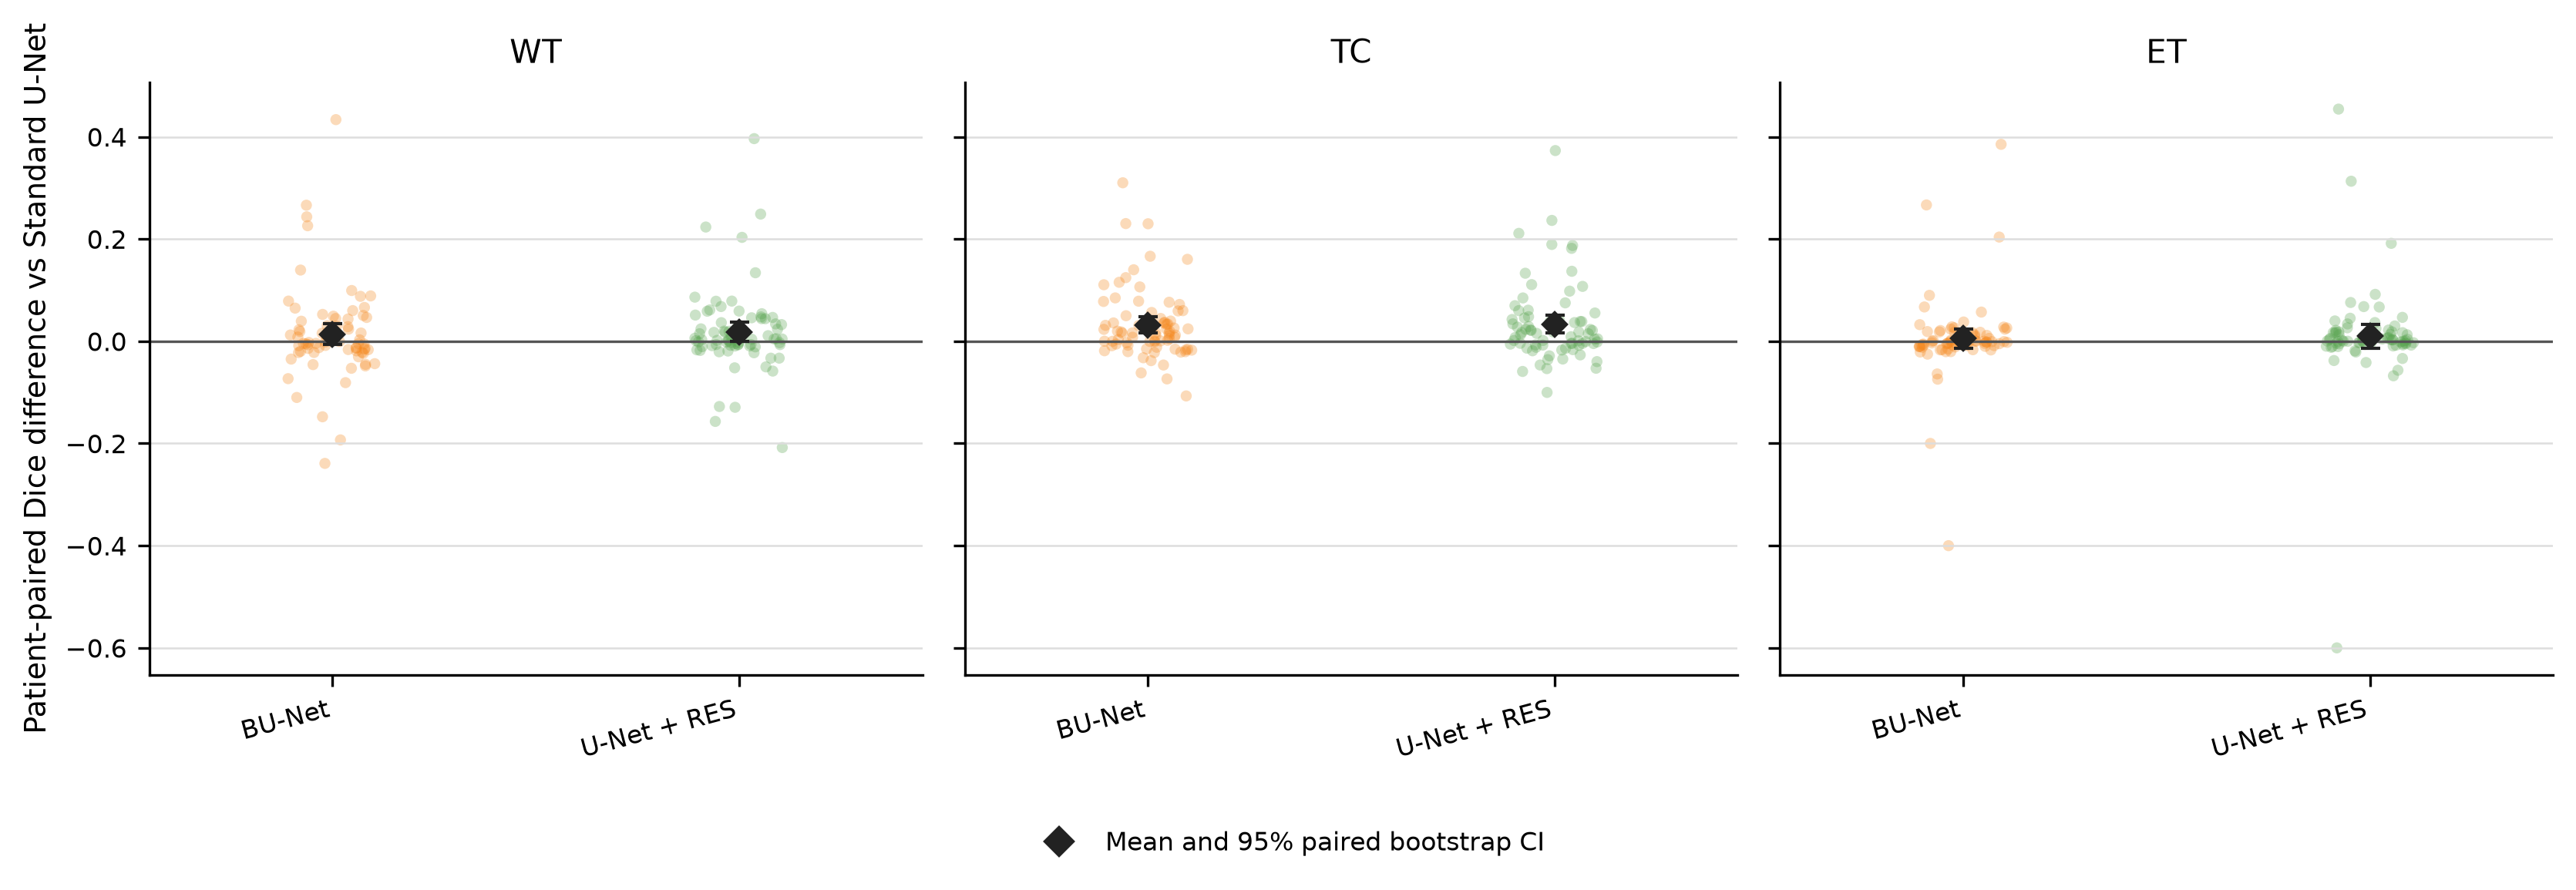
\includegraphics[width=0.92\linewidth,height=\textheight,keepaspectratio,alt={Figure 4. Patient-level paired regional Dice differences.}]{../figures/final/fig04_paired_region_differences.png}
\caption{Patient-level paired regional Dice
differences.}\label{fig:paired}
\end{figure}

\begin{figure}
\centering
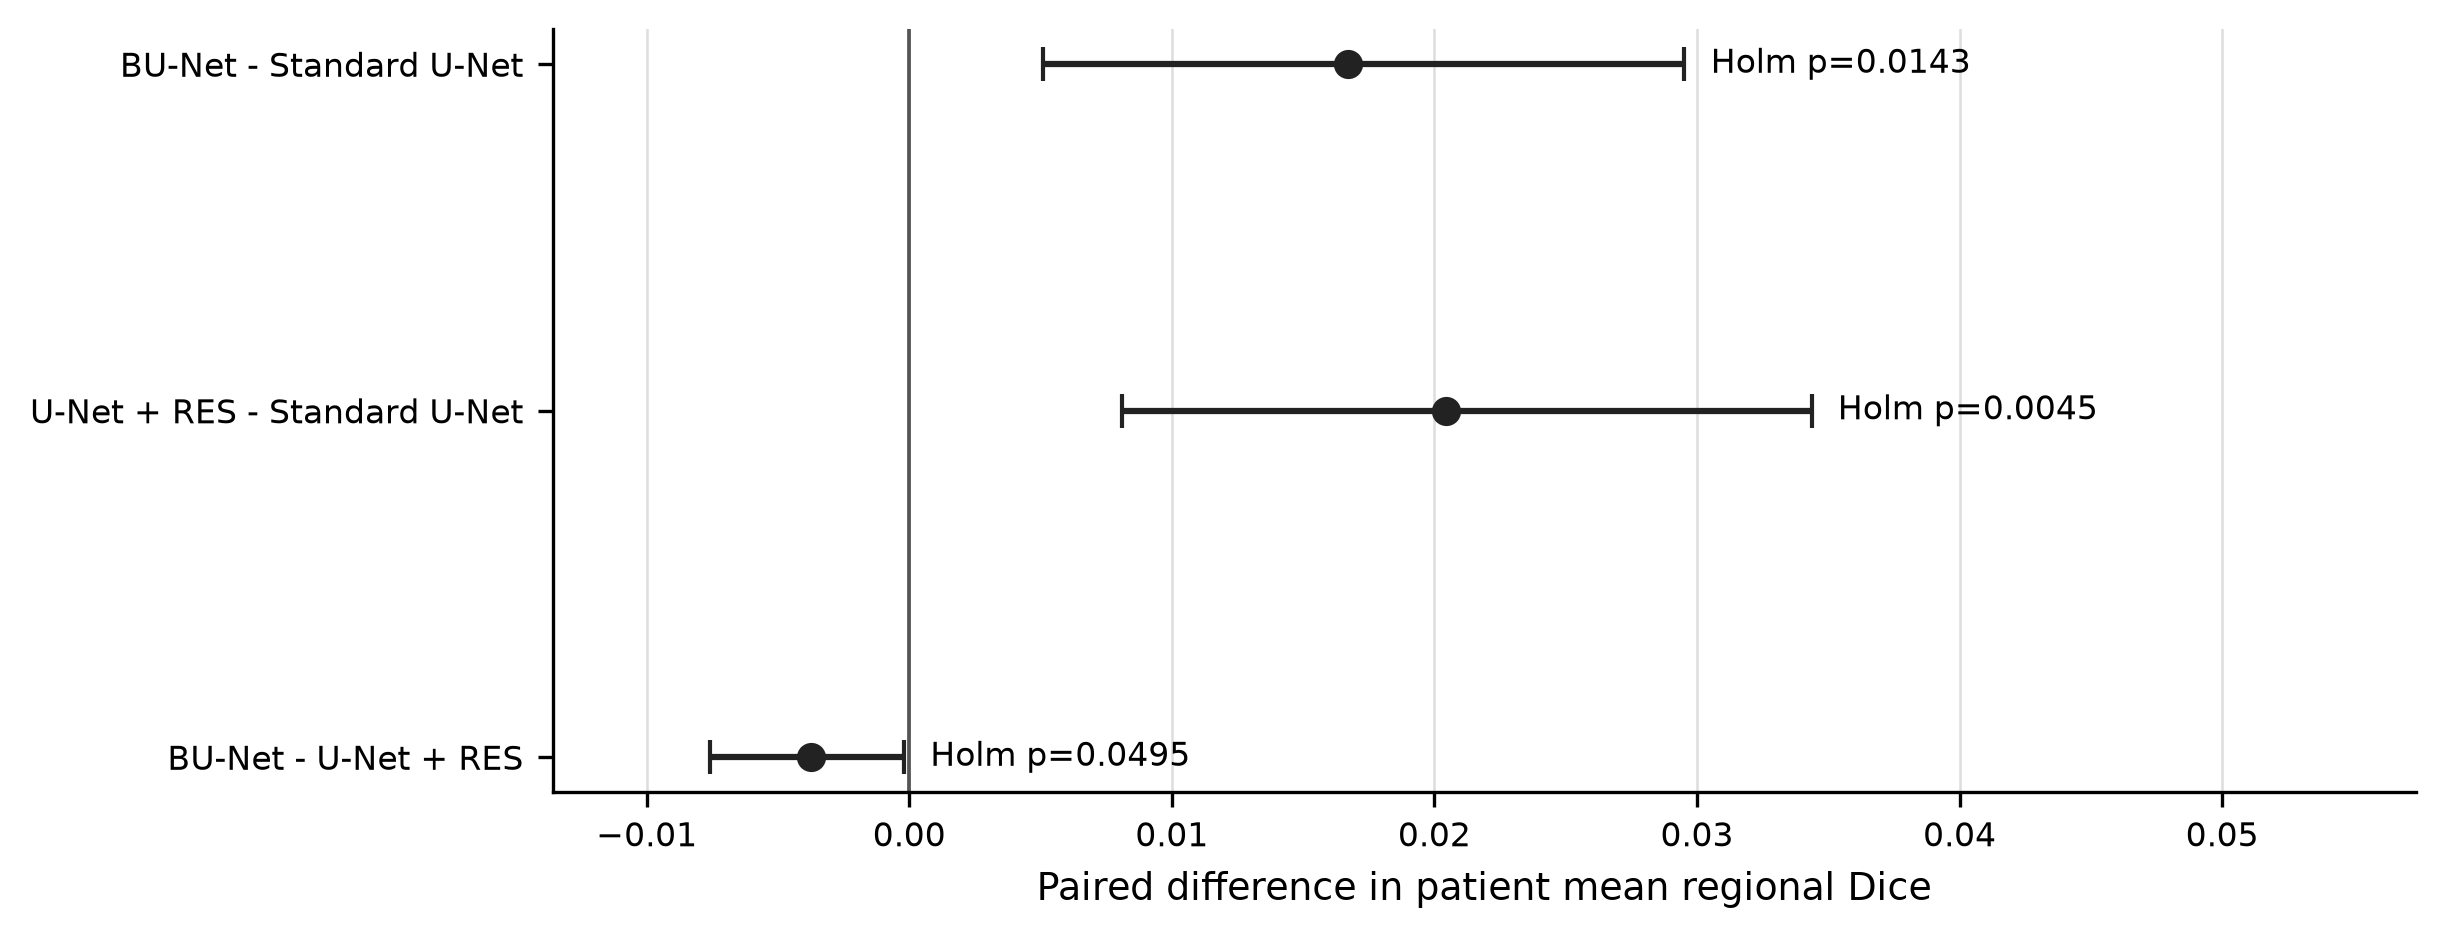
\includegraphics[width=0.92\linewidth,height=\textheight,keepaspectratio,alt={Figure 5. Frozen primary paired effects with 95\% bootstrap confidence intervals.}]{../figures/final/fig05_primary_effects.png}
\caption{Frozen primary paired effects with 95\% bootstrap
confidence intervals.}\label{fig:effects}
\end{figure}

\subsubsection{4.3 Regional, boundary, and lesion
estimates}\label{regional-boundary-and-lesion-estimates}

The largest regional overlap differences relative to standard U-Net
occurred for TC. ET overlap changed less. Surface Dice means favored
U-Net+RES numerically across all three regions. In contrast, finite HD95
means were lower for standard U-Net than for either component-based
model; several TC and ET observations were infinite because one mask was
empty. Thus, overlap improvements did not imply uniformly better
boundary outlier behavior.

\textbf{Table 6. Selected secondary outcomes. HD95 means use finite
observations; infinity counts are shown in parentheses.}

{\def\LTcaptype{none} % do not increment counter
\begin{longtable}[]{@{}
  >{\raggedright\arraybackslash}p{(\linewidth - 16\tabcolsep) * \real{0.1111}}
  >{\raggedright\arraybackslash}p{(\linewidth - 16\tabcolsep) * \real{0.1111}}
  >{\raggedright\arraybackslash}p{(\linewidth - 16\tabcolsep) * \real{0.1111}}
  >{\raggedright\arraybackslash}p{(\linewidth - 16\tabcolsep) * \real{0.1111}}
  >{\raggedright\arraybackslash}p{(\linewidth - 16\tabcolsep) * \real{0.1111}}
  >{\raggedright\arraybackslash}p{(\linewidth - 16\tabcolsep) * \real{0.1111}}
  >{\raggedright\arraybackslash}p{(\linewidth - 16\tabcolsep) * \real{0.1111}}
  >{\raggedright\arraybackslash}p{(\linewidth - 16\tabcolsep) * \real{0.1111}}
  >{\raggedright\arraybackslash}p{(\linewidth - 16\tabcolsep) * \real{0.1111}}@{}}
\toprule\noalign{}
\begin{minipage}[b]{\linewidth}\raggedright
Candidate
\end{minipage} & \begin{minipage}[b]{\linewidth}\raggedright
WT surface Dice
\end{minipage} & \begin{minipage}[b]{\linewidth}\raggedright
TC surface Dice
\end{minipage} & \begin{minipage}[b]{\linewidth}\raggedright
ET surface Dice
\end{minipage} & \begin{minipage}[b]{\linewidth}\raggedright
WT HD95 mm
\end{minipage} & \begin{minipage}[b]{\linewidth}\raggedright
TC HD95 mm
\end{minipage} & \begin{minipage}[b]{\linewidth}\raggedright
ET HD95 mm
\end{minipage} & \begin{minipage}[b]{\linewidth}\raggedright
ET lesion recall
\end{minipage} & \begin{minipage}[b]{\linewidth}\raggedright
ET lesion-wise Dice
\end{minipage} \\
\midrule\noalign{}
\endhead
\bottomrule\noalign{}
\endlastfoot
Standard U-Net & 0.605 & 0.577 & 0.734 & 21.9 & 17.4 (3 inf) & 14.8 (4
inf) & 0.470 & 0.356 \\
BU-Net & 0.621 & 0.586 & 0.744 & 35.8 & 22.0 (1 inf) & 16.8 (5 inf) &
0.475 & 0.367 \\
U-Net+RES & 0.637 & 0.595 & 0.748 & 31.9 & 21.0 (2 inf) & 16.9 (5 inf) &
0.476 & 0.370 \\
\end{longtable}
}

ET lesion recall was approximately 0.47 for all candidates, and ET
lesion-wise Dice remained below region-level ET Dice. These estimates
expose a lesion-detection limitation that a voxel-overlap summary alone
would obscure.

\subsubsection{4.4 Resource demand}\label{resource-demand}

BU-Net had 4.32 times the parameters and 3.87 times the MACs of standard
U-Net. U-Net+RES achieved the highest primary mean with 4.450 million
parameters, compared with 8.385 million for BU-Net. Its mean p50 latency
was 1.189 s/volume versus 1.258 s/volume, and its mean peak allocated
memory was 88.9 MB versus 234.8 MB. Development accelerator-hours per
run were similar and do not include preprocessing or study-level
engineering time.

\textbf{Table 7. Architecture and measured resource profile on one
host.}

{\def\LTcaptype{none} % do not increment counter
\begin{longtable}[]{@{}
  >{\raggedright\arraybackslash}p{(\linewidth - 16\tabcolsep) * \real{0.1111}}
  >{\raggedright\arraybackslash}p{(\linewidth - 16\tabcolsep) * \real{0.1111}}
  >{\raggedright\arraybackslash}p{(\linewidth - 16\tabcolsep) * \real{0.1111}}
  >{\raggedright\arraybackslash}p{(\linewidth - 16\tabcolsep) * \real{0.1111}}
  >{\raggedright\arraybackslash}p{(\linewidth - 16\tabcolsep) * \real{0.1111}}
  >{\raggedright\arraybackslash}p{(\linewidth - 16\tabcolsep) * \real{0.1111}}
  >{\raggedright\arraybackslash}p{(\linewidth - 16\tabcolsep) * \real{0.1111}}
  >{\raggedright\arraybackslash}p{(\linewidth - 16\tabcolsep) * \real{0.1111}}
  >{\raggedright\arraybackslash}p{(\linewidth - 16\tabcolsep) * \real{0.1111}}@{}}
\toprule\noalign{}
\begin{minipage}[b]{\linewidth}\raggedright
Candidate
\end{minipage} & \begin{minipage}[b]{\linewidth}\raggedright
Parameters, M
\end{minipage} & \begin{minipage}[b]{\linewidth}\raggedright
MAC/slice, G
\end{minipage} & \begin{minipage}[b]{\linewidth}\raggedright
FLOP/slice, G
\end{minipage} & \begin{minipage}[b]{\linewidth}\raggedright
p50 s/volume
\end{minipage} & \begin{minipage}[b]{\linewidth}\raggedright
p95 s/volume
\end{minipage} & \begin{minipage}[b]{\linewidth}\raggedright
Peak allocated MB
\end{minipage} & \begin{minipage}[b]{\linewidth}\raggedright
Development GPU-h/run
\end{minipage} & \begin{minipage}[b]{\linewidth}\raggedright
Mean regional Dice
\end{minipage} \\
\midrule\noalign{}
\endhead
\bottomrule\noalign{}
\endlastfoot
Standard U-Net & 1.943 & 2.676 & 5.353 & 0.492 & 0.528 & 67.0 & 0.332 &
0.736 \\
BU-Net & 8.385 & 10.344 & 20.688 & 1.258 & 1.285 & 234.8 & 0.384 &
0.752 \\
U-Net+RES & 4.450 & 9.459 & 18.919 & 1.189 & 1.215 & 88.9 & 0.388 &
0.756 \\
\end{longtable}
}

\begin{figure}
\centering
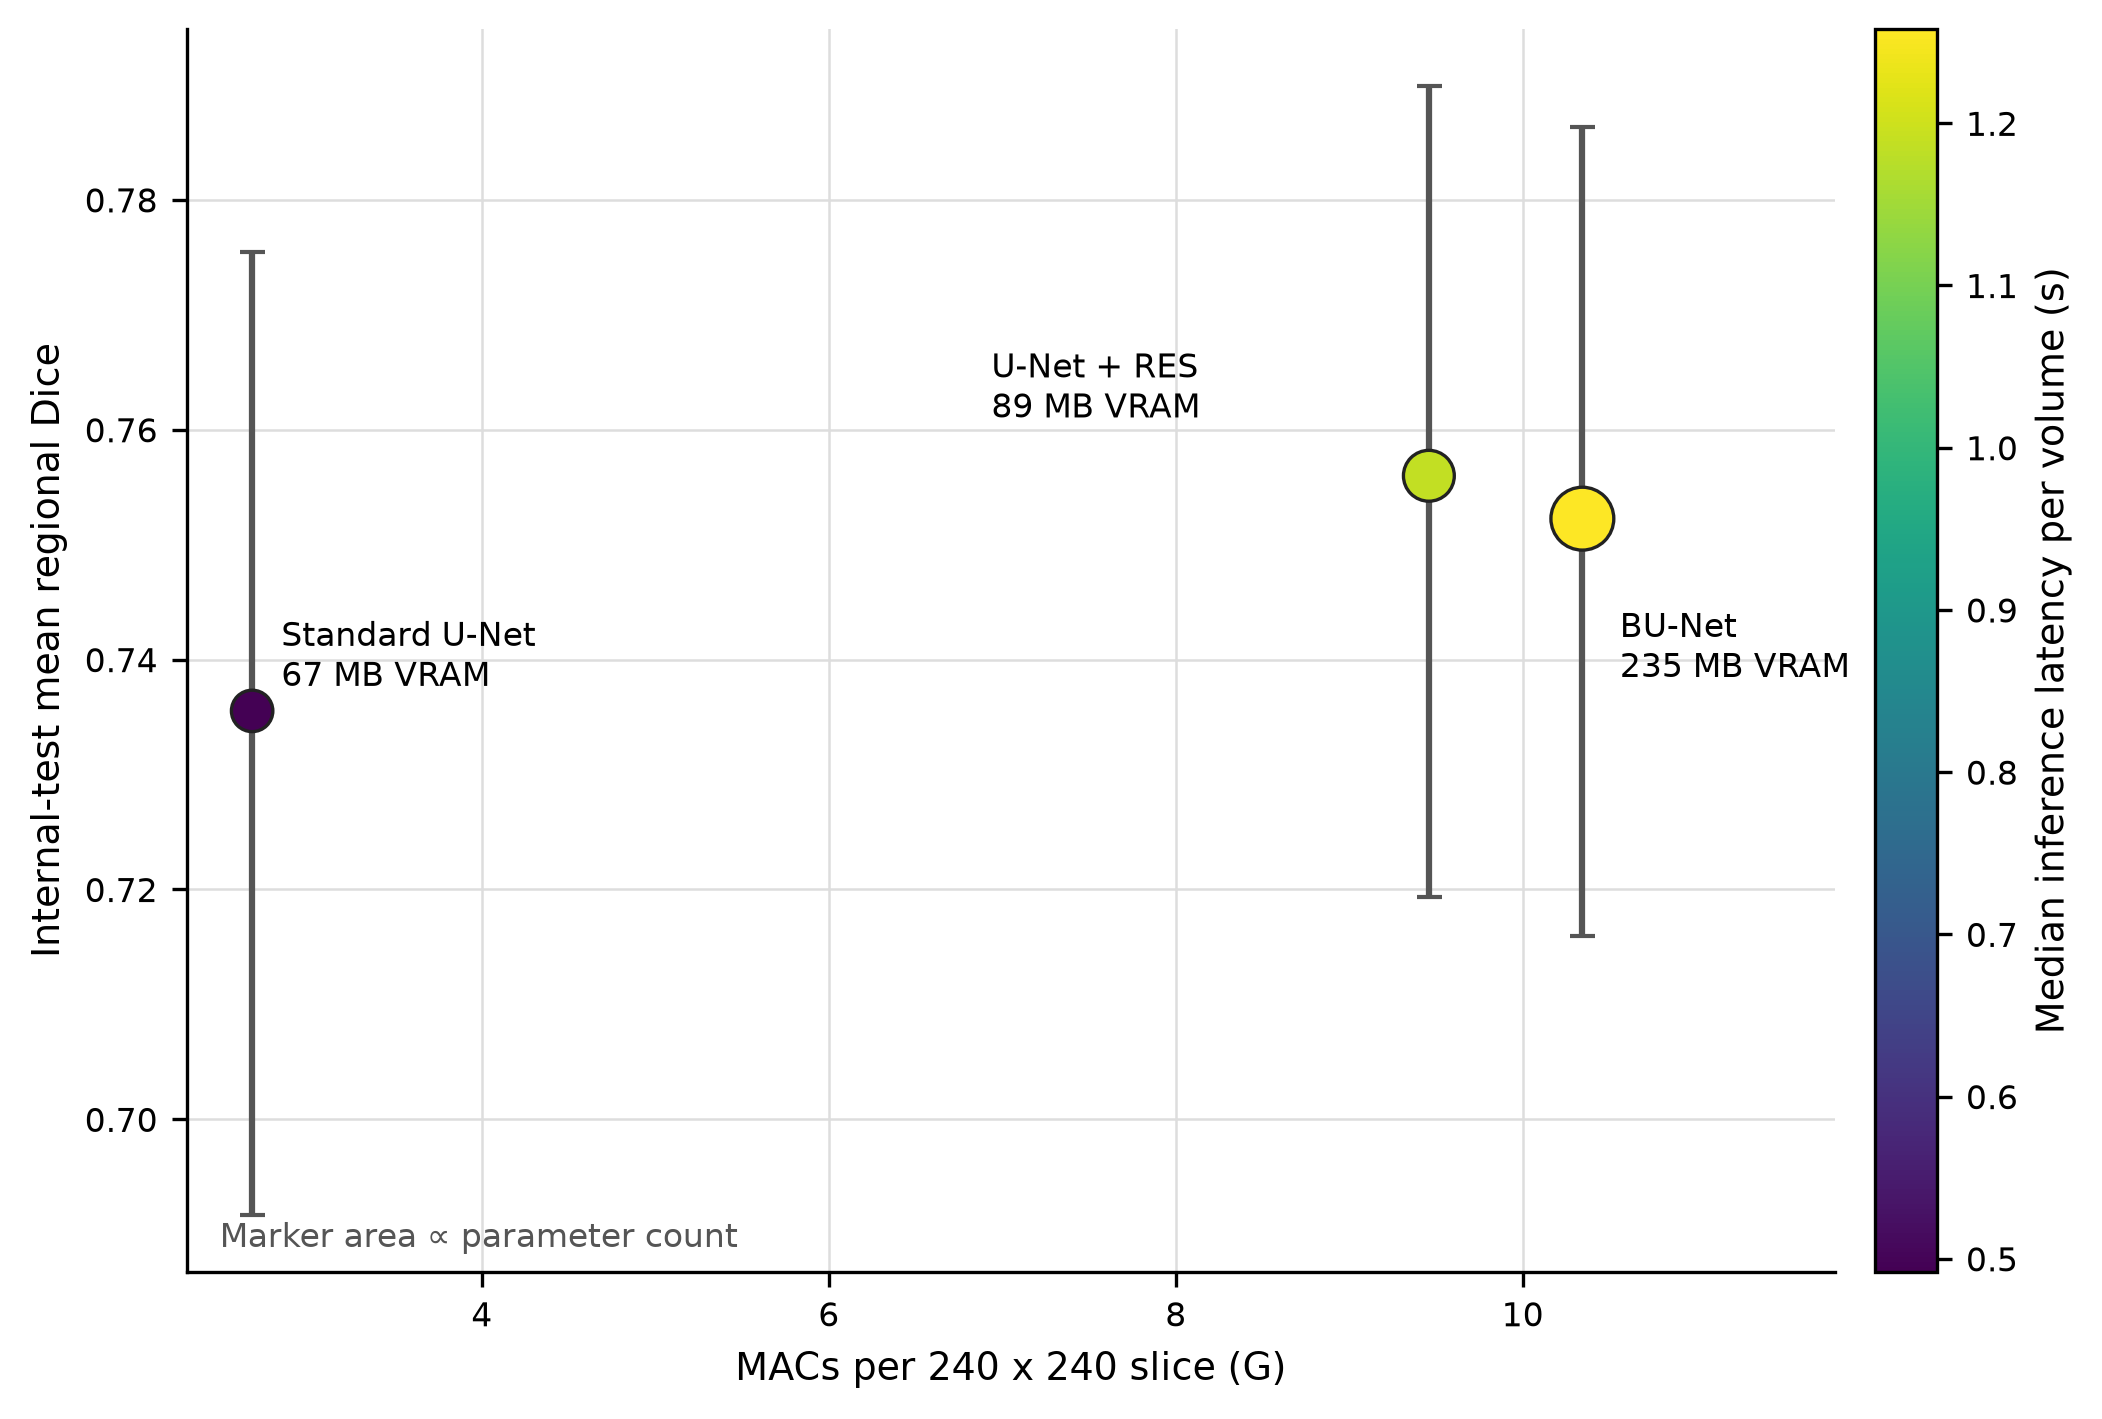
\includegraphics[width=0.92\linewidth,height=\textheight,keepaspectratio,alt={Figure 6. Mean regional Dice in relation to model and runtime resource measures.}]{../figures/final/fig06_performance_resource_tradeoff.png}
\caption{Mean regional Dice in relation to model and runtime
resource measures.}\label{fig:resources}
\end{figure}

\subsubsection{4.5 Exploratory subgroups and qualitative
review}\label{exploratory-subgroups-and-qualitative-review}

Exploratory subgroup estimates are reported without confirmatory p
values. HGG patients had higher mean scores than LGG patients for all
models. The ET-absent subset contained five patients and is descriptive
only. Training-set WT tertiles defined small (at most 64,267 mm3),
medium (64,267 to 123,163.3 mm3), and large burden groups.

\textbf{Table 8. Exploratory mean regional Dice by frozen subgroup.}

{\def\LTcaptype{none} % do not increment counter
\begin{longtable}[]{@{}
  >{\raggedright\arraybackslash}p{(\linewidth - 10\tabcolsep) * \real{0.1667}}
  >{\raggedright\arraybackslash}p{(\linewidth - 10\tabcolsep) * \real{0.1667}}
  >{\raggedright\arraybackslash}p{(\linewidth - 10\tabcolsep) * \real{0.1667}}
  >{\raggedright\arraybackslash}p{(\linewidth - 10\tabcolsep) * \real{0.1667}}
  >{\raggedright\arraybackslash}p{(\linewidth - 10\tabcolsep) * \real{0.1667}}
  >{\raggedright\arraybackslash}p{(\linewidth - 10\tabcolsep) * \real{0.1667}}@{}}
\toprule\noalign{}
\begin{minipage}[b]{\linewidth}\raggedright
Subgroup
\end{minipage} & \begin{minipage}[b]{\linewidth}\raggedright
n
\end{minipage} & \begin{minipage}[b]{\linewidth}\raggedright
Standard U-Net
\end{minipage} & \begin{minipage}[b]{\linewidth}\raggedright
BU-Net
\end{minipage} & \begin{minipage}[b]{\linewidth}\raggedright
U-Net+RES
\end{minipage} & \begin{minipage}[b]{\linewidth}\raggedright
Interpretation
\end{minipage} \\
\midrule\noalign{}
\endhead
\bottomrule\noalign{}
\endlastfoot
Grade: HGG & 59 & 0.806 & 0.808 & 0.812 & exploratory \\
Grade: LGG & 15 & 0.457 & 0.534 & 0.537 & exploratory \\
ET reference: present & 69 & 0.759 & 0.773 & 0.776 & exploratory \\
ET reference: absent & 5 & 0.418 & 0.470 & 0.480 &
descriptive\_insufficient\_n \\
WT burden: small & 24 & 0.713 & 0.735 & 0.746 & exploratory \\
WT burden: medium & 24 & 0.770 & 0.771 & 0.772 & exploratory \\
WT burden: large & 26 & 0.724 & 0.751 & 0.750 & exploratory \\
\end{longtable}
}

The qualitative panel includes preselected BU-Net success, hard, and
failure cases: BraTS20\_Training\_166 (ET Dice 0.924),
BraTS20\_Training\_137 (ET Dice 0.788), and BraTS20\_Training\_323 (ET
Dice 0.000). The failure case demonstrates that a favorable cohort mean
can coexist with near-zero ET overlap in an individual patient.
Modality, prediction, false-positive, and false-negative panels were
generated from retained test artifacts rather than selected after
manuscript inspection.

\begin{figure}
\centering
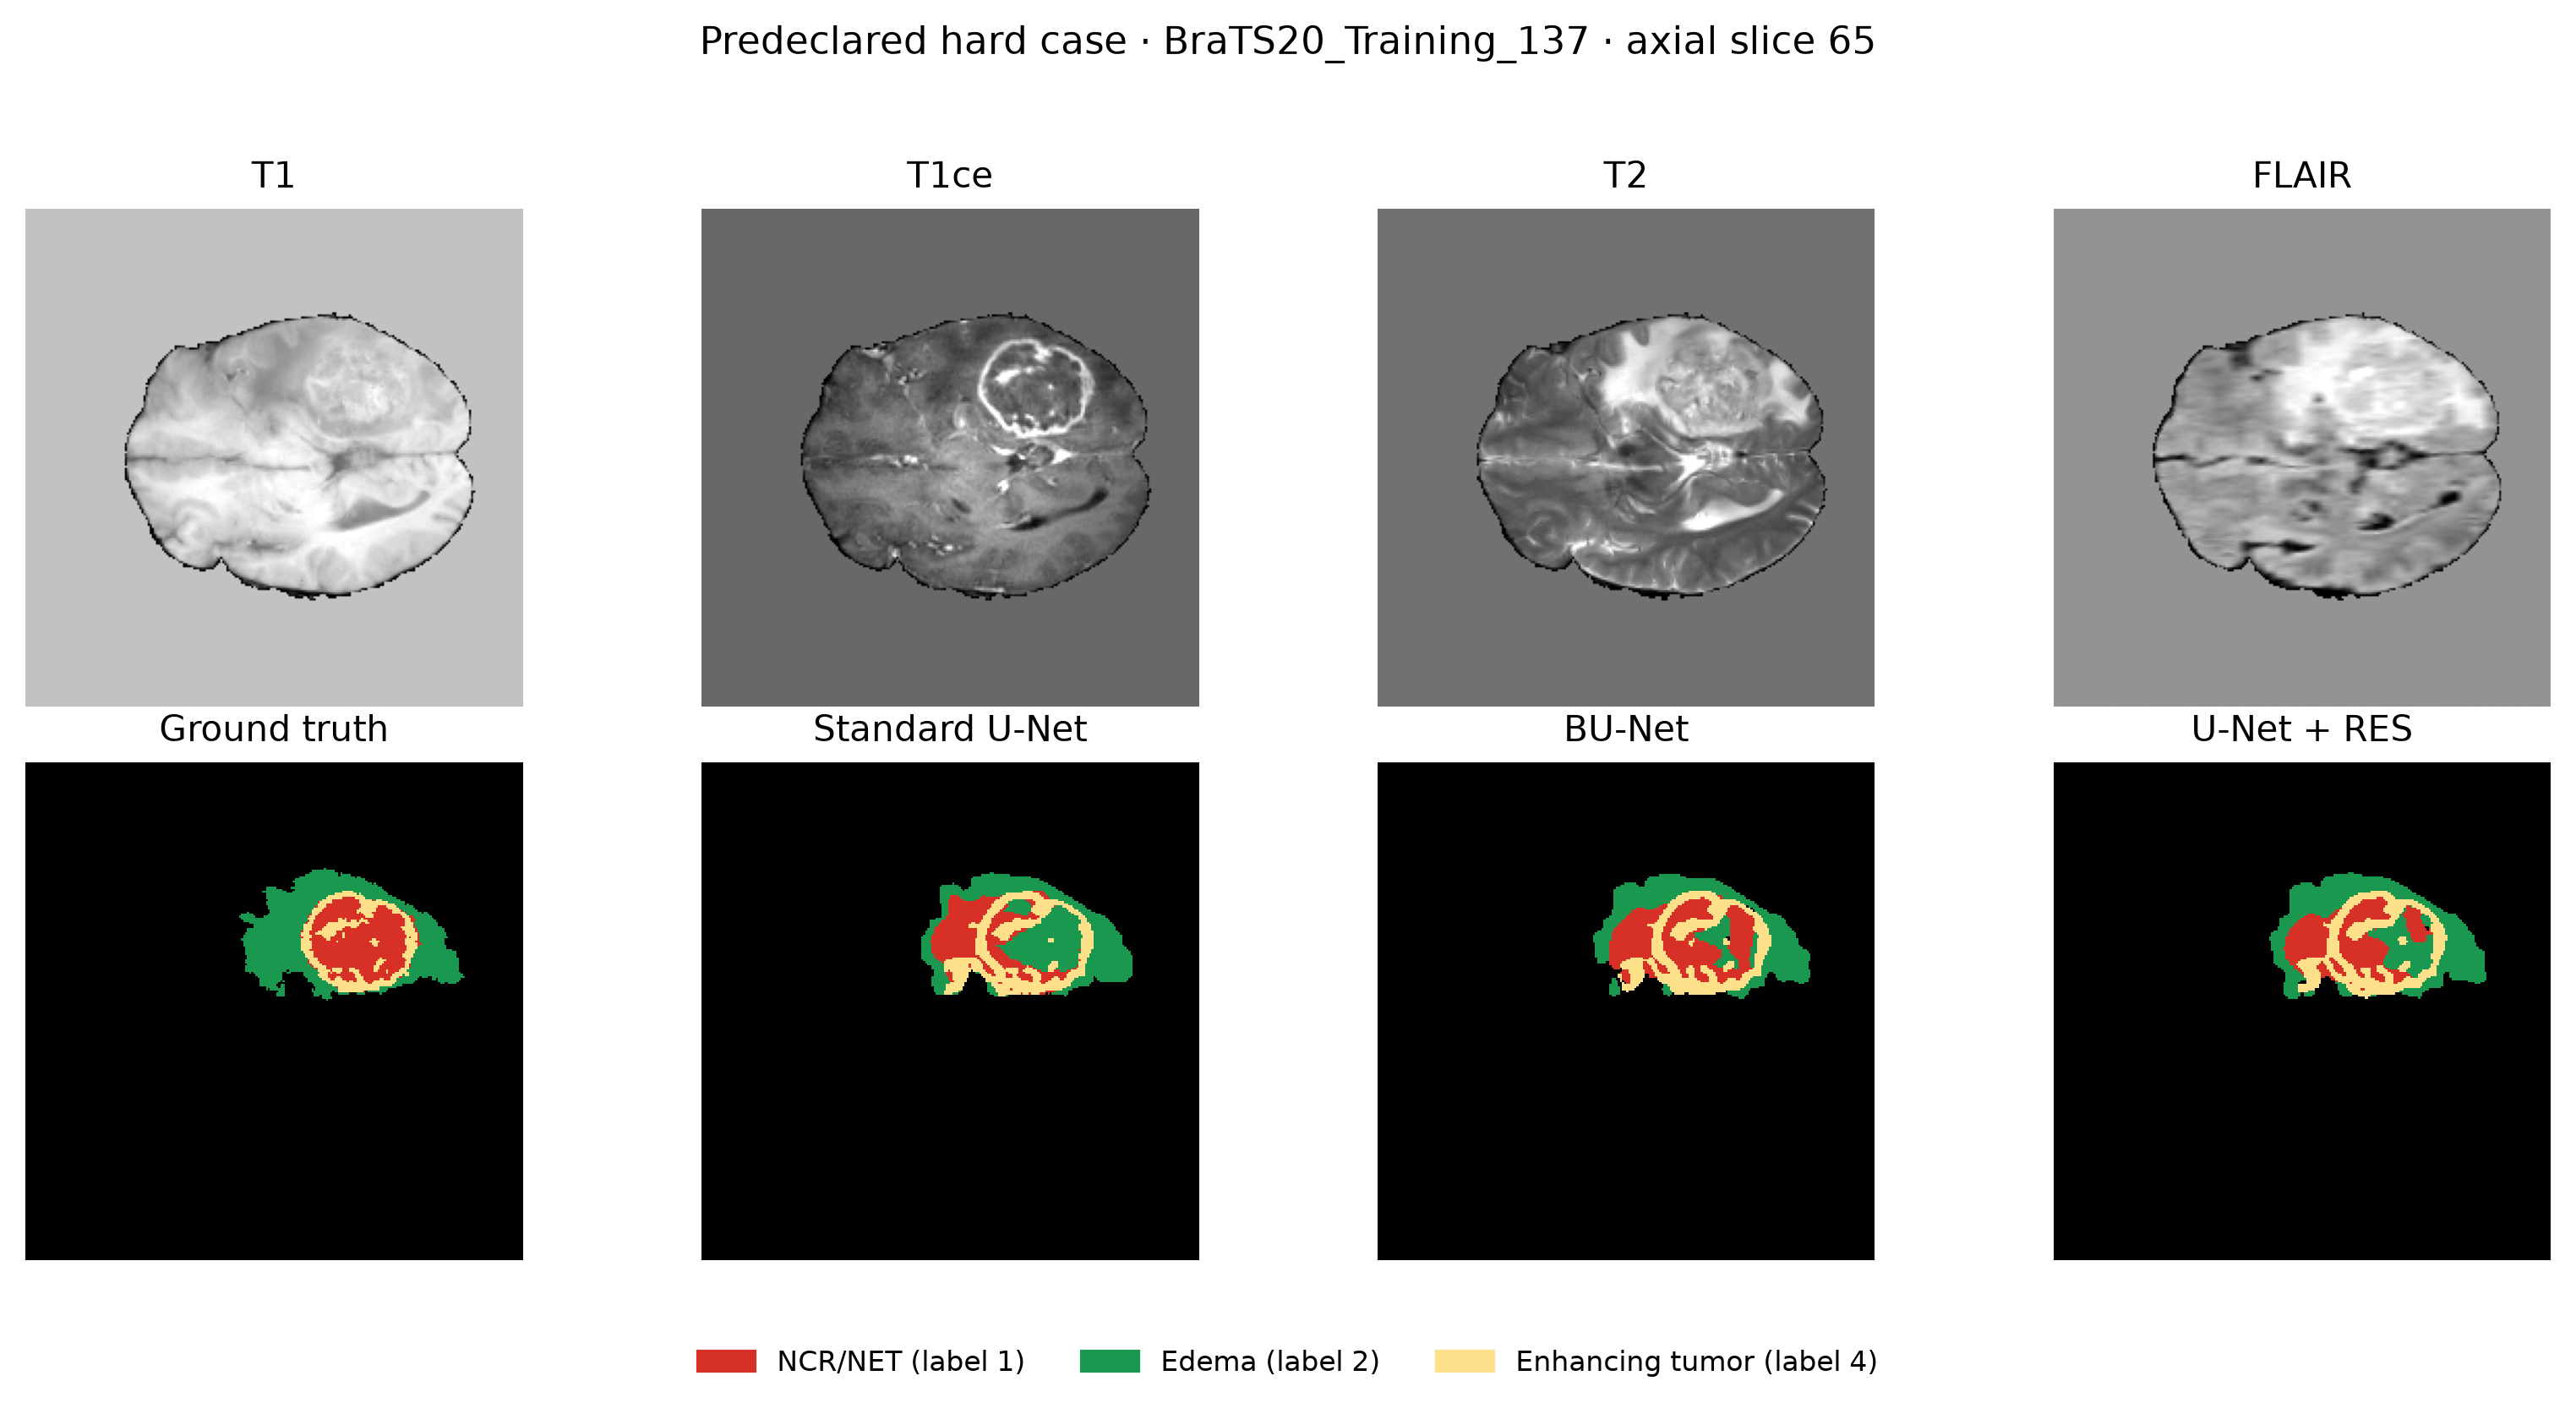
\includegraphics[width=0.92\linewidth,height=\textheight,keepaspectratio,alt={Figure 7. Multimodal MRI, reference labels, and frozen candidate predictions for an internal-test case.}]{../figures/final/fig07_modalities_and_predictions.png}
\caption{Multimodal MRI, reference labels, and frozen
candidate predictions for an internal-test case.}\label{fig:modalities}
\end{figure}

\begin{figure}
\centering
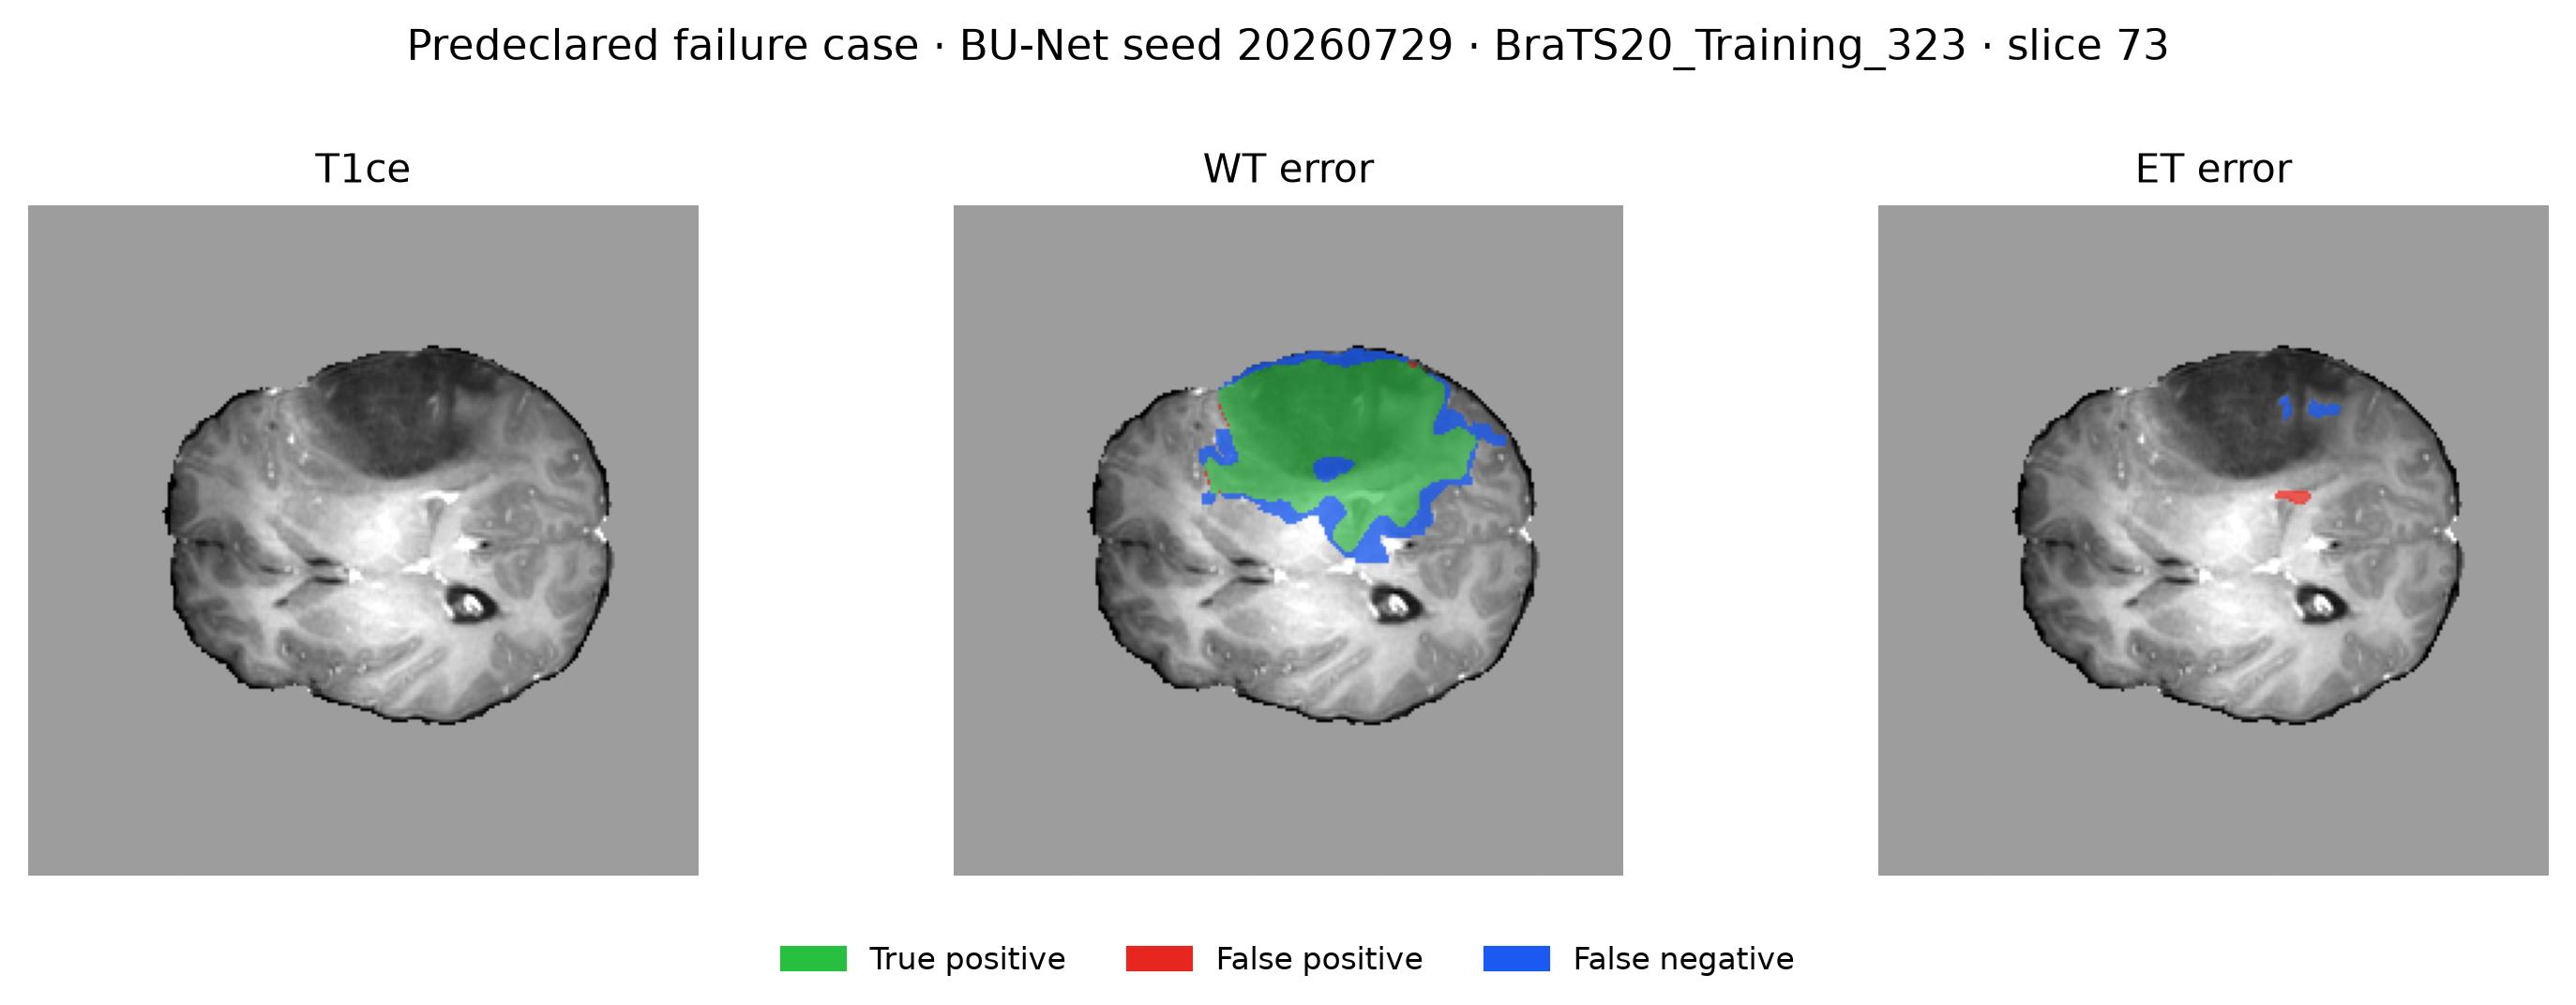
\includegraphics[width=0.92\linewidth,height=\textheight,keepaspectratio,alt={Figure 8. False-positive and false-negative error overlays.}]{../figures/final/fig08_false_positive_false_negative_overlay.png}
\caption{False-positive and false-negative error
overlays.}\label{fig:errors}
\end{figure}

\begin{figure}
\centering
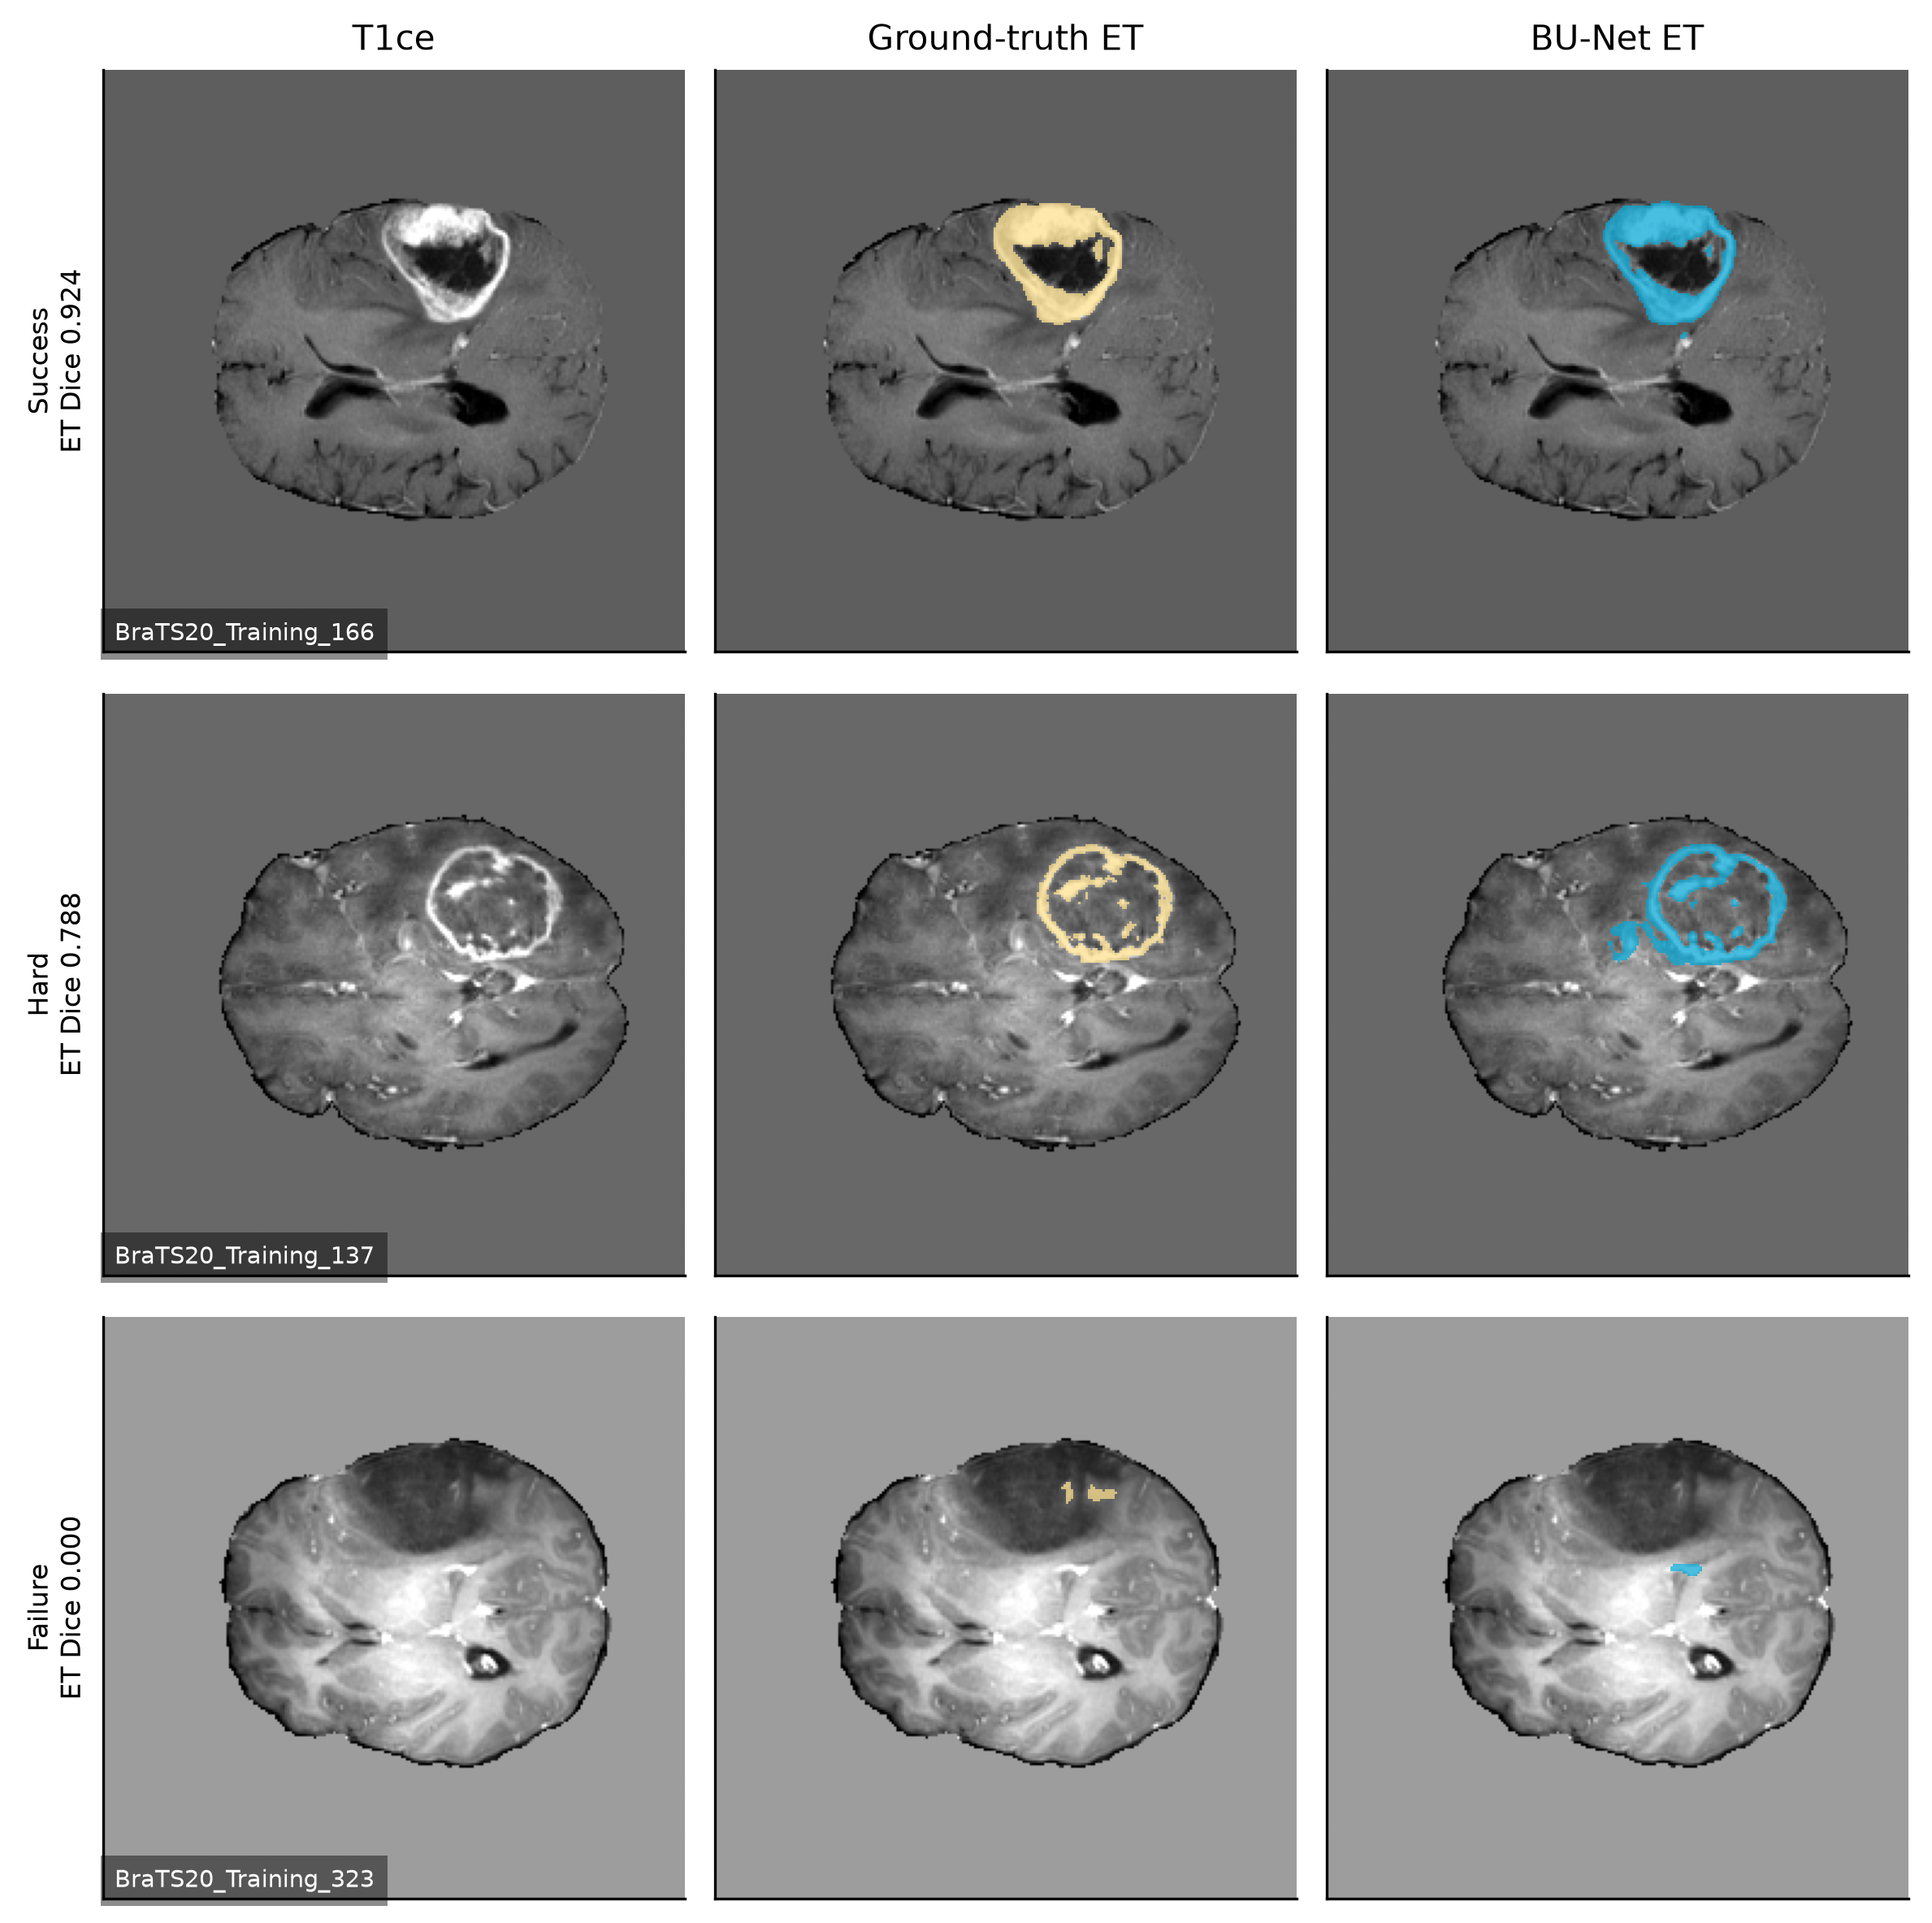
\includegraphics[width=0.92\linewidth,height=\textheight,keepaspectratio,alt={Figure 9. Prespecified BU-Net ET success, hard, and failure cases.}]{../figures/final/fig09_success_hard_failure_et_cases.png}
\caption{Prespecified BU-Net ET success, hard, and failure
cases.}\label{fig:cases}
\end{figure}

\begin{figure}
\centering
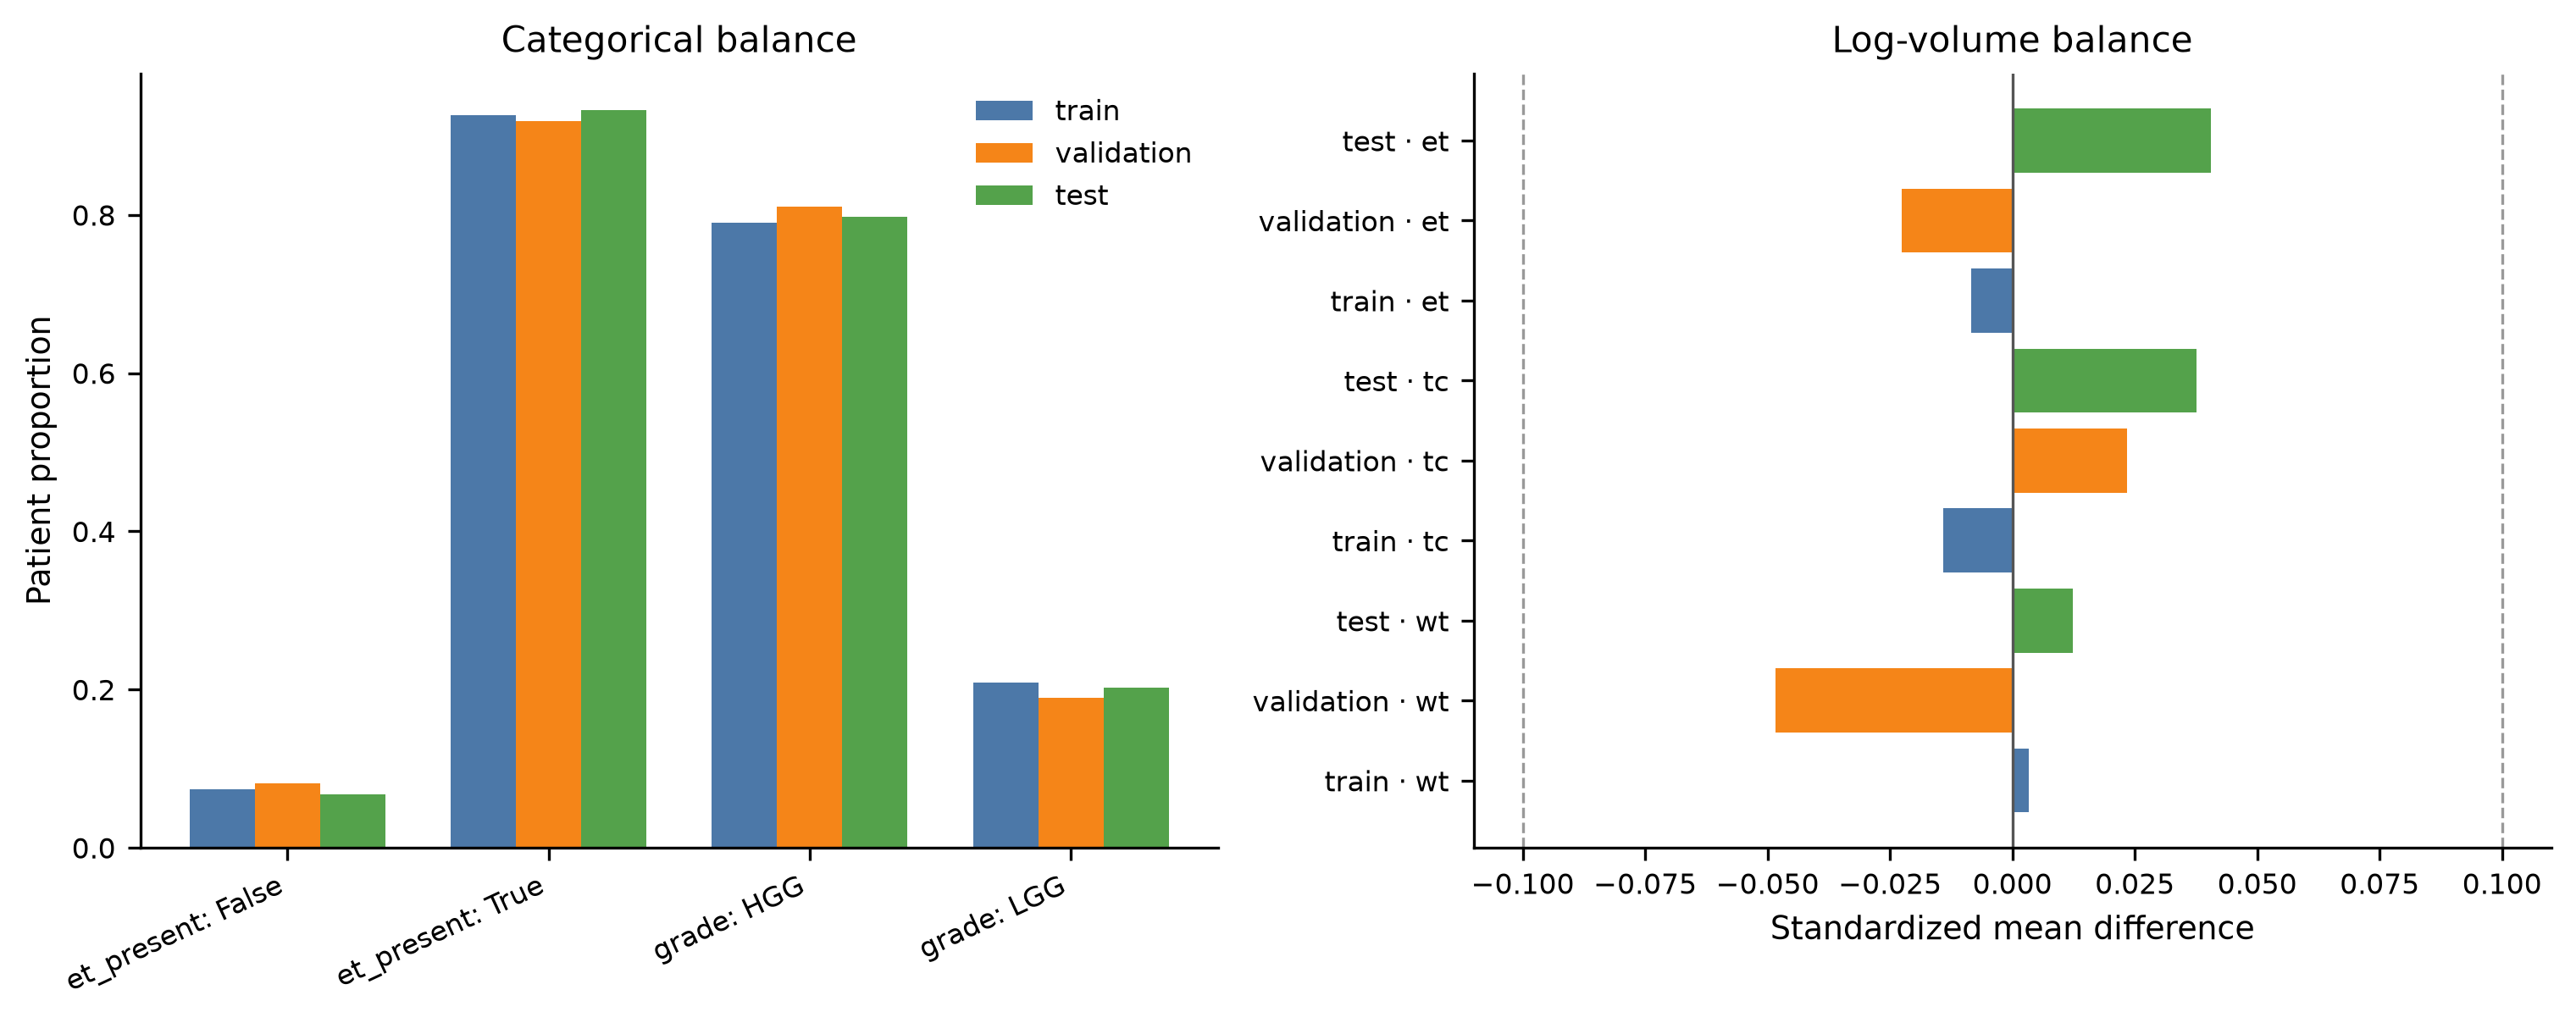
\includegraphics[width=0.92\linewidth,height=\textheight,keepaspectratio,alt={Supplementary Figure S1. Patient-level balance across frozen partitions.}]{../figures/final/figS01_split_balance.png}
\caption*{Supplementary Figure S1. Patient-level balance across frozen
partitions.}\label{fig:balance}
\end{figure}

\subsection{5. Discussion}\label{discussion}

\subsubsection{5.1 Principal findings}\label{principal-findings}

This controlled study supports three bounded conclusions. First, both
BU-Net and U-Net+RES produced small patient-level improvements in mean
regional Dice over standard U-Net after multiplicity correction. Second,
U-Net+RES slightly exceeded the full BU-Net on the frozen primary
endpoint. Third, BU-Net required substantially more parameters, MACs,
latency, and allocated memory than U-Net+RES. Under this implementation
and run budget, WC therefore did not provide an observable advantage
over RES alone.

The effect sizes were small. BU-Net's paired standardized effect versus
standard U-Net was +0.308, and the BU-Net versus U-Net+RES contrast was
-0.229. The latter p value was near 0.05 and its confidence interval lay
close to zero. The evidence should be interpreted as a
component-specific result under one bounded protocol, not a universal
claim that WC is ineffective.

\subsubsection{5.2 What the secondary outcomes
add}\label{what-the-secondary-outcomes-add}

Dice and surface Dice generally favored the component-based models, but
finite HD95 means did not. Standard U-Net had lower finite HD95 means in
WT, TC, and ET. This discordance can arise because Dice summarizes
overlap while HD95 emphasizes distant boundary errors and becomes
infinite when only one mask is empty. Reporting both prevents a
one-dimensional account of segmentation quality.

Lesion-level estimates also temper the voxel-level results. ET lesion
recall and lesion-wise Dice remained modest for every candidate. A model
can achieve a high regional Dice on a large focus while missing small
enhancing foci or generating disconnected false-positive components. The
qualitative failure case reinforces this limitation.

\subsubsection{5.3 Development ranking and test
behavior}\label{development-ranking-and-test-behavior}

BU-Net ranked first during five-seed development, but U-Net+RES ranked
first on the internal test. The development confidence interval between
the finalists included zero, so freezing both was important. Selecting
only the numerically leading validation model would have hidden this
uncertainty. The result illustrates why seed replication, frozen
finalist rules, and complete candidate reporting matter.

\subsubsection{5.4 Scope relative to broader segmentation
systems}\label{scope-relative-to-broader-segmentation-systems}

nnU-Net, TransBTS, nnFormer, and other 3D systems are relevant modern
comparators {[}9,14,15{]}. We did not train them. Nor did we perform
cross-dataset or multi-institutional external validation. Literature
scores cannot substitute for those experiments because acquisition,
cohort, preprocessing, compute, and evaluation rules differ. Our results
should therefore be read as a reproducible internal ablation of
published BU-Net components, not as a leaderboard or state-of-the-art
comparison.

\subsubsection{5.5 Limitations}\label{limitations}

This study has several limitations. It used one public dataset and an
internal split; external generalization is unknown. The networks were 2D
and cannot use through-plane context as a 3D model can. Training was
deliberately bounded at 2,000 optimizer steps or 0.5 accelerator-hours,
so the results do not describe fully converged scaling behavior. The
architecture widths and output encoding are reimplementation choices
rather than a bit-exact reproduction of BU-Net. Resource measurements
came from one Apple M1 Max host and do not establish deployment
performance on clinical hardware. The 1 mm surface tolerance was
predeclared but not calibrated against expert interobserver variability.
HGG/LGG labels were inherited from the challenge release and were not
independently adjudicated. Exploratory subgroups were small, especially
the five-patient ET-absent subset. Finally, no prospective workflow,
reader study, clinical endpoint, or regulatory assessment was performed.

\subsubsection{5.6 Reproducibility and
auditability}\label{reproducibility-and-auditability}

The released repository contains configuration files, split hashes,
model and loss code, evaluator tests, analysis scripts, machine-readable
outputs, figure and table generators, resource profiles, a claim ledger,
and a tracked-artifact manifest. A clean-clone reproduction report
records the exact commit and verifies deterministic output generation.
Raw BraTS data and model checkpoints are excluded because redistribution
is not authorized; users must obtain the dataset separately and
configure local paths.

\subsection{6. Conclusion}\label{conclusion}

In a leakage-safe, patient-level, multi-seed evaluation of three matched
2D U-Net-family candidates, the published BU-Net RES component improved
mean regional Dice relative to standard U-Net. Adding the published WC
component in the full BU-Net did not improve the primary endpoint over
RES alone and increased computational demand. Boundary and lesion-level
results were more mixed than overlap scores. The work provides
reproducible internal evidence about these components, while leaving 3D
comparison, external validation, clinical calibration, and prospective
utility as open questions.

\subsection{Data and code
availability}\label{data-and-code-availability}

Code, frozen manifests, derived reports, tables, figures, and
reproduction instructions are available at
https://github.com/TerekliTahaBerk/bratsarticle. BraTS images and labels
are not redistributed. Access to the original dataset is governed by the
BraTS data providers. The internal held-out test partition is a
study-specific subset of the BraTS 2020 training cohort and is not an
official challenge test set.

\subsection{Ethics statement}\label{ethics-statement}

This computational study used a publicly distributed, de-identified
challenge dataset and involved no direct participant contact or
intervention. Authors should confirm the final journal-specific
institutional review and exemption wording before submission.

\subsection{Declarations requiring author
confirmation}\label{declarations-requiring-author-confirmation}

Funding, competing interests, author contributions, and institutional
review wording were not inferable from the repository and must be
confirmed by the authors in the target journal's required format. No
declaration has been invented in this manuscript package.

\subsection{References}\label{references}

\begin{enumerate}
\def\labelenumi{\arabic{enumi}.}
\tightlist
\item
  Menze BH, et al.~The Multimodal Brain Tumor Image Segmentation
  Benchmark (BRATS). \emph{IEEE Transactions on Medical Imaging}.
  2015;34:1993-2024. doi:10.1109/TMI.2014.2377694.
\item
  Center for Biomedical Image Computing and Analytics. BraTS 2020 Tasks.
  University of Pennsylvania.
  https://www.med.upenn.edu/cbica/brats2020/tasks.html.
\item
  Bakas S, et al.~Advancing The Cancer Genome Atlas glioma MRI
  collections with expert segmentation labels and radiomic features.
  \emph{Scientific Data}. 2017;4:170117. doi:10.1038/sdata.2017.117.
\item
  Bakas S, et al.~Identifying the Best Machine Learning Algorithms for
  Brain Tumor Segmentation, Progression Assessment, and Overall Survival
  Prediction in the BRATS Challenge. arXiv:1811.02629. 2018.
\item
  Ronneberger O, Fischer P, Brox T. U-Net: Convolutional Networks for
  Biomedical Image Segmentation. \emph{MICCAI}. 2015.
  doi:10.1007/978-3-319-24574-4\_28.
\item
  Rehman ZU, et al.~BU-Net: Brain Tumor Segmentation Using Modified
  U-Net Architecture. \emph{Electronics}. 2020;9:2203.
  doi:10.3390/electronics9122203.
\item
  Salehi SSM, Erdogmus D, Gholipour A. Tversky Loss Function for Image
  Segmentation Using 3D Fully Convolutional Deep Networks.
  arXiv:1706.05721. 2017.
\item
  Abraham N, Khan NM. A Novel Focal Tversky Loss Function With Improved
  Attention U-Net for Lesion Segmentation. \emph{IEEE ISBI}. 2019.
  doi:10.1109/ISBI.2019.8759329.
\item
  Isensee F, Jaeger PF, Kohl SAA, Petersen J, Maier-Hein KH. nnU-Net: a
  self-configuring method for deep learning-based biomedical image
  segmentation. \emph{Nature Methods}. 2021;18:203-211.
  doi:10.1038/s41592-020-01008-z.
\item
  Maier-Hein L, et al.~Metrics Reloaded: recommendations for image
  analysis validation. \emph{Nature Methods}. 2024;21:195-212.
  doi:10.1038/s41592-023-02151-z.
\item
  Nikolov S, et al.~Clinically Applicable Segmentation of Head and Neck
  Anatomy for Radiotherapy: Deep Learning Algorithm Development and
  Validation Study. \emph{Journal of Medical Internet Research}.
  2021;23:e26151. doi:10.2196/26151.
\item
  Tejani AS, Klontzas ME, Gatti AA, Mongan JT, Moy L, Park SH, Kahn CE
  Jr.~Checklist for Artificial Intelligence in Medical Imaging (CLAIM):
  2024 Update. \emph{Radiology: Artificial Intelligence}.
  2024;6:e240300. doi:10.1148/ryai.240300.
\item
  Holm S. A Simple Sequentially Rejective Multiple Test Procedure.
  \emph{Scandinavian Journal of Statistics}. 1979;6:65-70.
  doi:10.2307/4615733.
\item
  Wang W, et al.~TransBTS: Multimodal Brain Tumor Segmentation Using
  Transformer. arXiv:2103.04430. 2021.
\item
  Zhou H-Y, et al.~nnFormer: Interleaved Transformer for Volumetric
  Segmentation. \emph{IEEE Transactions on Image Processing}.
  2023;32:4036-4049. doi:10.1109/TIP.2023.3293771.
\end{enumerate}

\end{document}
